\clearpage
\part*{Part XII. Decays And Nuclear Physics}
\label{atlaspart:12-decays-and-nuclei}
\addcontentsline{toc}{part}{Part XII. Decays And Nuclear Physics}
\section*{Introduction to Part XII}\label{narr:part:IX}
\addcontentsline{toc}{section}{Introduction to Part XII}
A body that is not a sink moves on. Part XII reads decay as exactly that, the forward edge of a non-sink in the move graph of the hub step, and then reads the rate, the prefactor, the lifetimes and the branching as counts and washed squares at the records of the release. The second half of the Part turns from decay to binding: the deuteron and the alpha as the pairing records of a joined web, the nuclear rows at the joined seeded web, and the processes of fission, fusion and the stellar bounds held as a table. The thread of the Part is the move graph of chapter 1-4 read at the sinks of chapter 1-5, and the dependency lines of its chapters point there and to the probe of chapter 1-6.

The order of the eight chapters separates two questions a textbook treats together, whether a body decays and how fast. The first chapter answers the first question with a graph: a body is stable exactly when it is a sink of the move graph, and a decay is a forward edge out of a non-sink. The three chapters that follow answer the second question with a count, the washed square of a read, and with the two objects that convert the count into a rate, the prefactor and the tick. The binding chapters then ask the same two questions of a joined web rather than a single body, and the answers there are open at every box, which the introduction says plainly so that the reader does not take a nuclear number from this Part. The reader should notice throughout that the construction has no transition amplitude: where the textbook sums amplitudes over final states, this Part counts records at a release and washes a square, and the difference is the subject of the prefactor open result of chapter 9-3.

Chapter 9-1 reads decay. Theorem~203.1 gives the process census against the eight derived moves, Theorem~203.3 states decay as the forward edge of a non-sink, Theorem~203.5 reads beta decay as the release at the plus-two arm and Open result~203.6 alpha decay as the cut at the many-body readout, with the decay graph as the census graph in Open result~203.2 and Open result~203.4; Open result~204.1 reads the release at the passed arm and Table~205.1 prints the decay board. The census of the forty-six process kinds of the literature against the eight moves types three as spelled, the muon decay at the hub step and its inverse and the binding and the fusion at the pairing move, eight as readouts and thirty-five as unspelled, Theorem~203.1. The move graph of the hub step and its inverse is an exact object whose decay edges release a cross-core pair, the literature decays are reached as paths at two of forty-one, the stable particles are sinks at all seven, and the first decay with no path is the tau to the down quark, which is the parting, Theorem~203.3. At the stop condition the seven stable bodies are sinks at six of seven with the gluon word a non-sink, the five lepton decays pass through the hub kind at both readings while the six quark decays part, and the register count rises at every forward edge and falls at every inverse edge, Open result~203.4. The plus-two arm of the neutron carries no forward edge, the neutron web being a sink with its forward set empty, so the beta rate cell is an output of the rate law at no non-sink, Theorem~203.5, and no joined nuclear web releases the alpha cluster under the cut move, the cut at the thirty-seven joined nuclear webs releasing a cluster isomorphic to the alpha web at none of the one hundred and thirteen cut edges, Open result~203.6. The decay board lists thirty-eight decay-rate targets at one line each, every process at its literature grade by name, with a derived cell at six of the lines and none at thirty-two, every cell an exact count per tick with the tick a name, Table~205.1.

Chapters 9-2 to 9-4 read the numbers of a decay. Theorem~206.1 reads the rate as the washed square of the read, Theorem~206.2 coherent release as the unwashed square at the joined web, Theorem~206.3 the decay rate as the imbalance readout, and Theorem~206.4 the branching ratios as the shares of the washed squares. The rate is the washed square of the read at two exact objects, the docking read of the photon at the electron dock with its square washed over the direction census, and the Compton object as that washed square over the electron Born square, Theorem~206.1. Coherent release stands at no admitted join and at the shared slot star beyond the valence bound alone, the washed square growing as the copy count at every join and the unwashed Born square as its square at the one-read matching alone, Theorem~206.2. Theorem~210.2 reads the prefactor as the tick width, with the prefactor from the record office width, Open result~210.1, open beside it: the prefactor read as the tick width multiplied by the office register is not an output of the derived rate cells, the tick width of the electron multiplied by the pinned register parting from the Compton objects at the first cell, Open result~210.1. Theorem~211.1 reads the imbalance readout with the lifetimes and the branching, and Theorem~211.2 reads the baryon asymmetry as the sign of the imbalance at the universe web, where the sign census of the forward edges carries a definite excess, the recorded forward edges of the horizon web at its first wave every one signed at the register count and the three sign readings agreeing at every edge, Theorem~211.2. A reader who wants the one place where the construction says why there is more matter than antimatter should read that box, and should notice that it is a sign and not a magnitude.

Chapter 9-5 holds alpha decay as a table, the table titled Alpha decay (chapter~\ref{mod:IX-5-alpha-decay}, among the instruments), awaiting the derivation of alpha decay as a forward edge of the move graph at the joined seeded webs. Chapter 9-6 reads binding: Open result~214.5 states binding as the pairing records at the deuteron and the alpha, with binding as the cross term of the joined first power, Open result~214.1, as the cross term at the two-vertex read, Open result~214.2, as the exact joined Born face, Open result~214.3, the nuclear web records at the joined stars, Open result~214.4, and the standing binding entry as the placement at the joined nuclear web, Open result~214.6, every one an open result with its parting named. The open results of this chapter are a single question asked at six faces, and the introduction gathers them so that the reader sees the shape of the question. The joined web at hydrogen carries a first power that exceeds the first powers of the bodies apart by a cross term at the order of the first powers themselves, while the binding at first order is the two-vertex term of the held chain, and the two differ at every face of the comparison, Open result~214.1. At the order-two read the dark set of the joined web is the union of the dark sets of the two bodies, so the cross term at that read is a rational multiple of the body terms with its root-six coordinate zero where the two-vertex term carries one, Open result~214.2. The deuteron and the alpha are exact objects at the register of the common support in the electron unit at both readings of the binding, the deuteron office parting at both register faces, and the order at which the ladder binding enters the office is the one open question, Open result~214.5. The complete four-star web is admitted at no composition under the valence bound, while the pairing object is common over every admitted pairing and the ratio of the four-cycle object to the triangle object equals the gain of one dark step, Open result~214.4. Chapter 9-7 reads the nuclear rows at the joined seeded web, Open result~216.1, where the proton sink of the bound-respecting seed joined with the neutron twin at the dock pairing saturates under the pairing move at the second wave to one sink of the neutral kind at two open docks, and chapter 9-8 holds fission, fusion and the stellar bounds as a table, the table titled Fission, fusion and stellar bounds (chapter~\ref{mod:IX-8-fission-fusion-and-stellar-bounds}, among the instruments).

In the language of the literature, this Part names decay, the decay rate, the lifetime, the branching ratio, beta and alpha decay, the baryon asymmetry, binding energy, the deuteron, the alpha particle, fission and fusion. The correspondence is by name at each. The boxes establish counts at a move graph and washed squares at the records of a release, and the binding chapter states that its results are open.

The dependency lines of the Part point to the moves and the saturation of Part I, to the probe of chapter 1-6, to the rate as a washed square read from the probability rule of Part III, and to the hub step of Part VIII, whose beta decay and boson widths are the same objects read from the other side. The binding chapters rest on hydrogen in Part VII, on the proton of Part IX and on the mass unit of Part X, and the baryon asymmetry rests on the horizon web of Part VI. A reader following the derivation graph will see Part XII as the Part that reads the move graph forward, where the Parts ahead of it read its sinks, and will see that every rate of the Part is a count per tick with the tick itself a name whose standing is the subject of chapter 10-10.
\section{Decay as the forward edge of a non-sink: the move graph of the hub step}\label{mod:IX-1-decay-as-the-forward-edge-of-a-non-sink-the-move-graph-of-the-hub-step}
\chdesig{12-1}{9-1}{IX-1-decay-as-the-forward-edge-of-a-non-sink-the-move-graph-of-the-hub-step}{IX-1-D538449-the-decay-board-release-one}
\label{narr:open:9-1}Decay is a forward edge. Theorem~203.1 gives the process census against the eight derived moves, Open result~203.2 and Open result~203.4 the decay graph as the census graph, Theorem~203.3 decay as the forward edge of a non-sink, Theorem~203.5 beta decay as the release at the plus-two arm, and Open result~203.6 alpha decay as the cut at the many-body readout; Open result~204.1 reads the release at the passed arm and Table~205.1 prints the decay board.
\begin{chconditional}[The process census against the eight derived moves]\label{box:IX-1-decay-as-the-forward-edge-of-a-non-sink-the-move-graph-of-the-hub-step:1}
Conditional on the results it rests on, each at its own standing. The census of the forty-six process kinds of the literature against the eight moves types three as spelled (the muon decay at the hub step and its inverse, the binding and the fusion at the pairing move), eight as readouts and thirty-five as unspelled, each with the move it would need named. The moves make ten of the seventeen tokens, unmake two, the muon leaf and the tau, and touch neither at seven: the hub step makes the muon from the electron and the tau from the muon, its inverse unmakes them into the lighter lepton and a released cross-core pair whose ends are the neutral bodies, and the pairing move makes the deuteron, the roster webs and the meson webs.
\end{chconditional}
\chstanding{conditional theorem}
\chdeps{Definitions 1.1 to 1.6, Open results 241.1 and 241.2, Theorems 241.3 and 241.4 and Open results 241.5 to 241.7 and Open results 245.1 and 245.2, Theorem 245.3, Open results 245.4 to 245.8 and Theorem 245.9}{Theorem 170.1 and Open result 170.2, Open result 204.1, Table 205.1 and Theorems 206.1 to 206.4}
\begin{chwall}[Decay graph as the census graph]\label{box:IX-1-decay-as-the-forward-edge-of-a-non-sink-the-move-graph-of-the-hub-step:2}
Under the anatomy map no literature decay is a path of the census graph and the stable particles are sinks at the up quark alone, while the key, the dark charges and the line functional agree at the two ends of twenty-one of the forty-one literature decays and differ at twenty, every charged-current decay through the W and the two photon modes of the Higgs.
\end{chwall}
\chstanding{open result}
\chdeps{Definitions 1.1 to 1.6, Open results 241.1 and 241.2, Theorems 241.3 and 241.4 and Open results 241.5 to 241.7 and Open results 245.1 and 245.2, Theorem 245.3, Open results 245.4 to 245.8 and Theorem 245.9}{Theorem 170.1 and Open result 170.2, Open result 204.1, Table 205.1 and Theorems 206.1 to 206.4}
\begin{chconditional}[Decay as the forward edge of a non-sink]\label{box:IX-1-decay-as-the-forward-edge-of-a-non-sink-the-move-graph-of-the-hub-step:3}
This conditional theorem, closing the open result of the previous releases at the order-two read through the hub, is stated once, as Theorem~158.1 of the chapter The hub step as the weak interaction, and this chapter cites it there without restating it.
\end{chconditional}
\chstanding{conditional theorem}
\chdeps{Definitions 1.1 to 1.6, Open results 241.1 and 241.2, Theorems 241.3 and 241.4 and Open results 241.5 to 241.7 and Open results 245.1 and 245.2, Theorem 245.3, Open results 245.4 to 245.8 and Theorem 245.9}{Theorem 170.1 and Open result 170.2, Open result 204.1, Table 205.1 and Theorems 206.1 to 206.4}
\begin{chwall}[Decay graph as the census graph at the stop condition]\label{box:IX-1-decay-as-the-forward-edge-of-a-non-sink-the-move-graph-of-the-hub-step:4}
At the stop condition the seven stable bodies are sinks at six of seven, the gluon word a non-sink; the five lepton decays pass through the hub kind at both readings, but the six quark decays part, their sources sinks, the register count rising at every forward edge and falling at every inverse edge.
\end{chwall}
\chstanding{open result}
\chdeps{Definitions 1.1 to 1.6, Open results 241.1 and 241.2, Theorems 241.3 and 241.4 and Open results 241.5 to 241.7 and Open results 245.1 and 245.2, Theorem 245.3, Open results 245.4 to 245.8 and Theorem 245.9}{Theorem 170.1 and Open result 170.2, Open result 204.1, Table 205.1 and Theorems 206.1 to 206.4}
\begin{chtheorem}[Beta decay as the release at the plus-two arm]\label{box:IX-1-decay-as-the-forward-edge-of-a-non-sink-the-move-graph-of-the-hub-step:5}
This theorem, closing the open result of the previous releases at the literal closure reading, is stated once, as Theorem~170.1 of the chapter Beta decay and the boson widths, and this chapter cites it there without restating it.
\end{chtheorem}
\chstanding{theorem}
\chdeps{Definitions 1.1 to 1.6, Open results 241.1 and 241.2, Theorems 241.3 and 241.4 and Open results 241.5 to 241.7 and Open results 245.1 and 245.2, Theorem 245.3, Open results 245.4 to 245.8 and Theorem 245.9}{Theorem 170.1 and Open result 170.2, Open result 204.1, Table 205.1 and Theorems 206.1 to 206.4}
\begin{chwall}[Alpha decay as the cut at the many-body readout]\label{box:IX-1-decay-as-the-forward-edge-of-a-non-sink-the-move-graph-of-the-hub-step:6}
No joined nuclear web releases the alpha cluster under the cut move: at the thirty-seven joined nuclear webs the cut releases a cluster isomorphic to the alpha web at none of the one hundred and thirteen cut edges, every roster chain carrying its two neutron stars at its ends.
\end{chwall}
\chstanding{open result}
\chdeps{Definitions 1.1 to 1.6, Open results 241.1 and 241.2, Theorems 241.3 and 241.4 and Open results 241.5 to 241.7 and Open results 245.1 and 245.2, Theorem 245.3, Open results 245.4 to 245.8 and Theorem 245.9}{Theorem 170.1 and Open result 170.2, Open result 204.1, Table 205.1 and Theorems 206.1 to 206.4}
The process kinds are laid at their literature grade by name, every kind typed by its bindings against the moves at both readings, and the moves that make and unmake each token read off the move graph of the hub step and the pairing move. The census rests on the hub step, the pairing move, attach and join, the hub-forming move, the dock read, the carrier records, the two neutral objects and the mixing result, with the readouts, the typed count and the relabelling result at their own premises. The open questions are recorded beside the census. The theorem and the rate results of the next chapter rest on them or re-meet them, and the rate, the prefactor and the lifetimes stand at the next three chapters.
\begin{chbridge}
In the standard account an unstable particle decays through an interaction term of the Lagrangian, its rate the golden rule \cite{Dirac1927,Fermi1934}, and a stable particle has no channel open below its mass. The correspondence is by name.
\end{chbridge}
\begin{chproof}[finite computation with its exact part]
\textit{The premises.} The axiom and the six definitions of Section~\ref{mod:FRAMEWORK}, definitions. The moves of Section~\ref{mod:I-4-moves-in-one-table}, definitions. The sinks of the saturation of Section~\ref{mod:I-5-saturation-in-one-figure-seeds-waves-termination-sinks}, a theorem. The library of webs, a material. The literature table of decays and stable particles, by name. The chain from the axiom to this result is five chapters deep.

\textit{The exact part: the move graph and one of its edges.} The vertices are the bodies of the grammar among the webs of the library and every web one hub step away from them. A forward edge is a hub step applied at a site of a vertex (pure at every site, or freed at every link of a saturated site by the cut, the deletion or the pair), and an inverse edge removes a hub with its leaf pair, removing or keeping the odd leg by its state and restoring the freed link at the pair-inverse. A decay edge, at the reading adopted, is an inverse edge releasing a cross-core pair, two cross cores per released pair. The smallest instance, drawn at the figure, is the muon decay. From the muon web (the leaf form with its hubs) and the inverse of the hub step at its hub, by removing the hub with its leaf pair, we obtain the two-dock electron web and one released cross-core pair, whose two ends are the two neutral bodies. This is the first of four matching paths and the one literature decay reached at the first vertex.

\textit{The finite computation.} The input objects are the sixty-four webs of the library, forty-nine of them bodies of the grammar and fifteen over the valence bound (the uniform chains), and the literature table of forty-one decays, seven stable particles and fifteen forbidden decays by their web tokens. The enumeration rule builds the graph as the closure of the forward and inverse hub steps from the bodies, capped at one step away from the library. The totals at the natural checkpoint are
\begin{equation} \adjustbox{max width=\dimexpr\linewidth-3em\relax}{$\displaystyle \begin{gathered} 502\ \text{vertices}\ (34\ \text{library webs},\ 3\ \text{neutral},\ 468\ \text{one step away}), \\ 2138\ \text{edges}\ (1069\ \text{forward},\ 1069\ \text{inverse}), \end{gathered}$} \end{equation}
the edges typed by their release (the link freed 1688, the open leg 268, the hub-leg pair 84, the cross-core pair 48, the kept leg 26, the leaf pair 24), and the decay edges at the reading adopted 24. The test applied to each literature decay is whether its source and products stand as a path of decay edges, and to each stable particle whether its web is a sink (no forward edge). The aggregation is the count. The decays reached as paths are 2 of 41, the muon decay first. The stable particles are sinks at 7 of 7, the up quark and the electron first. The forbidden decays are paths at 0 of 15. The first decay with no path is the tau to the down quark, where a path of sixteen steps exists but the two cross-core pairs released, doubled, equal the two neutral products at none. At the reading beside (every inverse edge a decay edge, one cross core per pair) the counts are 2 of 41, 1 of 41 and the sinks 4 of 7. The production edges beside number 651, of which 431 are bodies, over the forty bodies carrying a (2,4) leg.

\textit{The check.} The decay-graph result of the preceding reading is re-met at its cells. The four alterations of the construction (the reading of the decay edge, the cap on the step count, the release typing and the sink rule) each move the counts they name, and striking the text moves every cell. The result was reproduced by an independent route, two engines of different construction agreeing at every cell at both runs and at six of six pieces of the cross-comparison.
\chcert{49}
\end{chproof}
\begin{figure}[h]
\centering
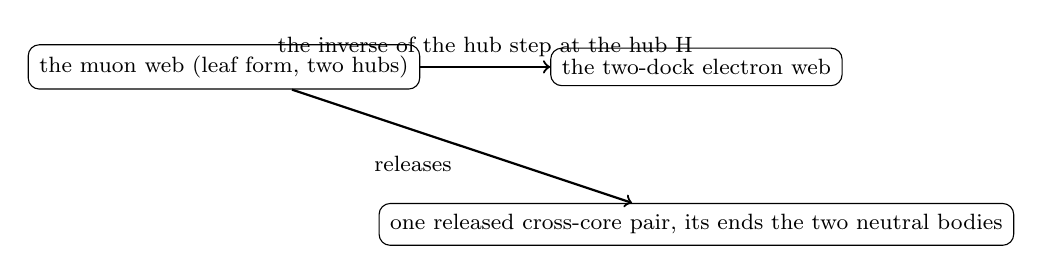
\begin{tikzpicture}[every node/.style={font=\footnotesize}]
\node[draw,rounded corners,inner sep=4pt] (mu) at (0,0) {the muon web (leaf form, two hubs)};
\node[draw,rounded corners,inner sep=4pt] (e) at (6,0) {the two-dock electron web};
\node[draw,rounded corners,inner sep=4pt] (p) at (6,-2) {one released cross-core pair, its ends the two neutral bodies};
\draw[->,thick] (mu) -- node[above] {the inverse of the hub step at the hub H} (e);
\draw[->,thick] (mu) -- node[below left] {releases} (p);
\end{tikzpicture}
\caption{The muon decay as the first decay edge of the move graph. The inverse of the hub step at the hub of the muon web removes the hub with its leaf pair, leaving the two-dock electron web and releasing one cross-core pair whose two ends are the two neutral bodies.}
\end{figure}
\section{The release at the passed arm}\label{mod:IX-1-D538074-w-rpar}
\begin{chwall}[The release at the passed arm]\label{box:IX-1-D538074-w-rpar:1}
This result re-poses the stop reading of the decay graph at every body with a dock and locates the arms, the passed records and the rate at the release as outputs of the tables already derived. Face A, every unstable body of the roster a non-sink at its passed arm with its release equal to its closure and its rate an exact cell, reads no at the eleven unstable bodies. Non-sinks at their passed arms two of eleven, the release equal to the closure one of eleven, the rate exact three of eleven, every clause met at none. Face B reads yes, and the parting is named. The first unstable body whose release parts from its closure is the muon, its release in the closure currency against its derived closure differing by the closure of the four links the measuring path traverses. The second parting the neutron, releasing nothing at its typing with its arms capped at twelve of twelve, the closure equal at zero against zero. And the top, the W, the Z, the Higgs and the four quark words carry no measuring path, having no dock assigned.
\end{chwall}
\chstanding{open result}
\chdeps{Definitions 1.1 to 1.6, Theorem 195.1 and Theorem 203.1, Open result 203.2, Theorem 203.3, Open result 203.4, Theorem 203.5 and Open result 203.6}{no theorem beyond it at this release}
The arms of every body with a dock are located from the decay graph at its stop reading, the passed records are read along the measuring path, the release is summed in the closure currency and compared body by body with the closure cell of the body-alone office, and the rate is read at the release where the body is a non-sink at its passed arm. The result rests on the premises of its derivation, the beta release at the plus-two arm, the rate law, the branching result, the lifetime hierarchy, the decay graph at the stop condition, the read-count question, the count as the leading term, the premise census, the body-alone result, the cross-term theorem, the boson widths, the alpha cut, the unstable-row correction, the neutron through the deuteron, the dark-end body, the bound-respecting seed, the roster, the fission and fusion result, the W office and the proton-web seeds, each read as it stands.
\begin{chbridge}
The decay rate of an unstable body is the squared matrix element of the transition summed over the final states and multiplied by the phase space. The correspondence is by name.
\end{chbridge}
\begin{chproof}[finite computation with its census and its exact part]
\textit{The premises.} The axiom and the six definitions of Section~\ref{mod:FRAMEWORK}, definitions. The body-alone office rule of Section~\ref{mod:VIII-2-body-alone-office-rule}, a theorem. The move graph of the hub step of Section~\ref{mod:IX-1-decay-as-the-forward-edge-of-a-non-sink-the-move-graph-of-the-hub-step}, an open result consumed at its sinks. The twenty results the reading paragraph names at their own standings. The chain from the axiom to this result is seven chapters deep.

\textit{The exact part: the release at one body.} At a body with an entry dock, the measuring path is the union of the geodesics from the entry to the nearest hubs. The arms are the links off the path, sorted at the hubs and the junction (the cross at a stop hub, the plus-two arm at a hub off the path, the junction at the (3,3) links). The records the path passes at each arm are counted as the measures of its links. From the arms, by the cut that turns every link of an arm down, we obtain the measure released. From the per-link closure cells of the body-alone office summed over the links of the arms, we obtain the release in the closure currency. The identity
\begin{equation}
\text{arms}+\text{path}+\text{docks}=\text{the derived closure}
\end{equation}
holds at 5 of 5 reads of the five bodies. The smallest instance is the neutron, listed at the figure, with three arms of measures $44$, $27$ and $32$ and every passed link capped at 12 of 12, so the release is zero against the closure zero, equal. The base result is re-met at its plus-two arm (the site with its dock, the four links of measure $32$, the arm-removal readout $2592$ and the cell $1024/17\,689$). At the muon the release in the closure currency is
\begin{equation}
\tfrac{3\,006\,289\,413}{655\,360\,000}+\tfrac{661}{225}\sqrt{2}+\tfrac{1675}{262\,144}\sqrt{3}
\quad\text{against the closure}\quad
\tfrac{27\,214\,907\,303}{5\,898\,240\,000}+\tfrac{661}{225}\sqrt{2}+\tfrac{6\,301\,957}{294\,912\,000}\sqrt{3},
\end{equation}
the difference the closure of the four links the path traverses, $\tfrac{79\,151\,293}{2\,949\,120\,000}+\tfrac{2\,208\,791}{147\,456\,000}\sqrt{3}$, the dock term zero.

\textit{The census and the computation.} The set counted is the seventy-four primary webs of the decay graph at the stop condition, every anatomy found at its source table and re-met at the measure, the dressing and the first power at 74 of 74. The property tested is whether a web carries a measuring path (an entry dock assigned at the five bodies, the first dock in the written site order elsewhere). A path stands at 18 of 74 and none at 56. At every web with a path the rate at the release is the washed square of the released readouts (the measure released multiplied by the dressing, squared and summed over the arms) over the Born square of the first power,
\begin{equation}
\text{rate}=\frac{\sum_{\text{arms}} (m_{\text{released}}\, d)^{2}}{S_1^{2}} ,
\end{equation}
exact at 18 of 18, the muon $3217/11\,449$, the tau $1651/7203$, the neutron $527/2527$ at every link and $0$ at its typing, and the proton $145/729$ at every link and $0$ at its typing. At the eleven unstable bodies of the roster the counts are as follows. Non-sinks at their passed arms 2 of 11 (the muon and the tau, releasing the measures $65$ and $139$), the release equal to the closure 1 of 11 (the neutron, at zero against zero), the rate an exact cell 3 of 11, every clause met at 0 of 11. The first parting is the muon, parting from its closure by the path term.

\textit{The check.} Arming the proton moves its release. Striking the arms moves every rate while the stop reading is re-met at every sink. Striking the closure of the muon moves its parting. Leaving the Born square unsquared moves every rate. Each alteration moves the cells it names. The result was reproduced by an independent route, two engines of different construction agreeing at every cell at both runs, with the rate law re-built at 56 of 56 rows, the shares at 36 of 36 and the first powers and prefactors at 13 of 13 as the controls.
\chcert{74}
\end{chproof}
\begin{figure}[h]
\centering
\begin{adjustbox}{max width=\linewidth}\begin{tabular}{lll}
\hline
arm of the neutron & where it stands & measure of its links \\
\hline
the cross & at the hub H & 44 \\
the junction & at the (3,3) links & 27 \\
the plus-two arm & at the site $Q_2$ with its dock $n_2$, four links & 32 \\
\hline
\end{tabular}\end{adjustbox}
\caption{The three arms of the neutron at its stop reading, every passed link capped at the typing adopted, so that the neutron releases nothing and its release equals its closure at zero against zero.}
\end{figure}
\section{The decay board and its comparisons}\label{mod:IX-1-D538449-the-decay-board-release-one}
\begin{chtable}[The decay board]\label{box:IX-1-D538449-the-decay-board-release-one:1}
The decay board lists thirty-eight decay-rate targets at one line each, every process at its literature grade by name, with a derived cell at six of the lines and none at thirty-two, every cell an exact count per tick with the tick a name. The lifetime in ticks and the implied tick by provenance are rendered at every cell, the comparison word is ratio-only at the six lines with a cell and none at the rest, no cell carrying a unit by provenance, and the ratios of the cells against the ratios of the observed widths part at every pair by many orders.
\end{chtable}
\chstanding{instrument}
\chdeps{Definitions 1.1 to 1.6, Theorem 203.1, Open result 203.2, Theorem 203.3, Open result 203.4, Theorem 203.5 and Open result 203.6 and Theorems 211.1 and 211.2}{no theorem beyond it at this release}
The targets are listed one per line, the derived cells are read where a result supplies one, the lifetimes in ticks and the implied ticks are rendered by provenance, the comparison words are typed from the cells and the units, the precision ledger is laid at every line, and the board is rendered last from the tables. It is a tabulation at its counts, built from the release at the passed arm and rebuilt from its parents, the nuclear half-lives to follow.
\begin{chbridge}
The lifetimes and the partial widths of the unstable bodies are tabulated with their uncertainties, the lifetime of a body the inverse of its total width and the branching fraction of a channel its partial width over the total, each entry the result of a measurement at a stated precision \cite{Fermi1934,Weinberg1967}. The correspondence is by name.
\end{chbridge}
\begin{chproof}[instrument table]
\textit{The rule that produced the table.} Every target of the targets file stands at one line in the file order, thirty-eight lines, each process given by its name. The sink assigned is assigned by the row map at ten of the thirty-eight (the five bodies at their sinks, the photon, the W, the Z, the Higgs and the top at their library word names) and none at the twenty-eight meson and baryon lines, where no identification of a library word with a meson or a baryon stands. The assigned cell is the arm-release cell at the typing adopted where the sink carries a read assigned, else the rate-law total where a rate-law line stands, else none. The lifetime in ticks is one over the cell. The comparison word is ratio-only where a cell stands and none elsewhere, inside at none and outside at none, since no cell carries a unit by provenance. The columns of the table below are the line, the sink assigned and the assigned cell as an exact count per tick. The observed lifetimes, widths and uncertainties are kept at the board, apart from the derived cells.

\begin{center}
\begin{adjustbox}{max width=\linewidth}\begin{tabular}{lll}
\hline
line & sink derived & cell derived, a count per tick \\
\hline
the electron & the two-dock web, a sink at the stop reading & $1108/4489$ \\
the proton & the bound-respecting sink & $0$ at the typing adopted ($145/729$ at every link) \\
the muon & the leaf form, a non-sink & $3217/11\,449$ \\
the tau & the leaf form, a non-sink & $1651/7203$ \\
the neutron & the neutron seed, a sink & $0$ at the typing adopted ($527/2527$ at every link) \\
the Higgs & the Higgs word & $121/16$ at the rate law \\
the thirty-two other lines & none or no measuring path & none \\
\hline
\end{tabular}\end{adjustbox}
\end{center}

\textit{The counts of the table.} The lines number 38 of 38, a sink is assigned at 10 of 38, a derived cell stands at 6 of 38 and none at 32 of 38, fourteen cell lines stand over the readings, and the comparison word is ratio-only at 6 of 38 and none at 32 of 38. The ratios of the cells against the ratios of the observed widths parting at 7 of 7 pairs by six to fifteen orders and within an order at 0 of 7. The rate-law totals at the muon $35\,734/11\,449$ and the tau $26\,963/21\,609$ equal to the branching totals at 10 of 10, the shares summing to one at 10 of 10, and the prefactor equal to one over the first power squared at 13 of 13. The result was reproduced by an independent route, two engines agreeing at every table, and the board file cites every table at 11 of 11.
\end{chproof}
\par\medskip\noindent{\itshape Decay read as an edge, the next chapter reads its rate.}\label{narr:close:9-1}\par
\section{The rate as the washed square of the read and the tick unit}\label{mod:IX-2-rate-as-the-washed-square-of-the-read-and-the-tick-unit}
\chdesig{12-2}{9-2}{IX-2-rate-as-the-washed-square-of-the-read-and-the-tick-unit}{IX-2-D543234-w-nmvt}
\label{narr:open:9-2}Theorem~206.1 reads the rate as the washed square of the read, Theorem~206.2 coherent release as the unwashed square at the joined web, Theorem~206.3 the decay rate as the imbalance readout, and Theorem~206.4 the branching ratios as the shares of the washed squares.
\begin{chconditional}[The rate as the washed square of the read]\label{box:IX-2-rate-as-the-washed-square-of-the-read-and-the-tick-unit:1}
Conditional on the results it rests on, each at its own standing. The rate is the washed square of the read at two exact objects: the docking read of the photon at the electron dock has its square washed over the direction census, the Compton object is that washed square over the electron Born square, and the pair-creation objects per genre are the duplicate and delete counts of the conservation result over the genre register, every object an exact rational.
\end{chconditional}
\chstanding{conditional theorem}
\chdeps{Definitions 1.1 to 1.6, Theorems 18.1 to 18.4 and Open results 18.5 and 18.6, Theorems 28.1 and 28.2, Open results 28.3 and 28.4 and Theorem 28.5 and Theorem 203.1, Open result 203.2, Theorem 203.3, Open result 203.4, Theorem 203.5 and Open result 203.6}{Theorem 170.1 and Open result 170.2, Open result 208.1, Open result 209.1, Open result 210.1 and Theorem 210.2, Theorems 211.1 and 211.2 and Theorem 254.1}
\begin{chconditional}[Coherent release as the unwashed square at the joined web]\label{box:IX-2-rate-as-the-washed-square-of-the-read-and-the-tick-unit:2}
Conditional on the results it rests on, each at its own standing. The coherent release stands at no admitted join and at the shared slot star beyond the valence bound alone: the washed square grows as the copy count at every join and the unwashed Born square as its square at the one-read matching alone, so the growth ratio reads the copy count at the shared star and one at the admitted joins.
\end{chconditional}
\chstanding{conditional theorem}
\chdeps{Definitions 1.1 to 1.6, Theorems 18.1 to 18.4 and Open results 18.5 and 18.6, Theorems 28.1 and 28.2, Open results 28.3 and 28.4 and Theorem 28.5 and Theorem 203.1, Open result 203.2, Theorem 203.3, Open result 203.4, Theorem 203.5 and Open result 203.6}{Theorem 170.1 and Open result 170.2, Open result 208.1, Open result 209.1, Open result 210.1 and Theorem 210.2, Theorems 211.1 and 211.2 and Theorem 254.1}
\begin{chconditional}[The decay rate as the imbalance readout]\label{box:IX-2-rate-as-the-washed-square-of-the-read-and-the-tick-unit:3}
Conditional on the results it rests on, among them rate as the washed square of the read, coherent release as the unwashed square at the joined web, first power as the act readout sum, decay graph as the census graph at the stop condition, the unstable row correction as the open move readout and prefactor from record office width, each at its own standing. The rate form is a theorem at every non-sink with the prefactor by construction: each of the thirteen non-sinks of the decay graph carries a forward edge, the prefactor is one over the Born square of the first power at the hub rule, an exact rational, and the implied prefactor of every derived rate cell equals the construction.
\end{chconditional}
\chstanding{conditional theorem}
\chdeps{Definitions 1.1 to 1.6, Theorems 18.1 to 18.4 and Open results 18.5 and 18.6, Theorems 28.1 and 28.2, Open results 28.3 and 28.4 and Theorem 28.5 and Theorem 203.1, Open result 203.2, Theorem 203.3, Open result 203.4, Theorem 203.5 and Open result 203.6}{Theorem 170.1 and Open result 170.2, Open result 208.1, Open result 209.1, Open result 210.1 and Theorem 210.2, Theorems 211.1 and 211.2 and Theorem 254.1}
\begin{chconditional}[The branching ratios as the shares of the washed squares]\label{box:IX-2-rate-as-the-washed-square-of-the-read-and-the-tick-unit:4}
Conditional on the results it rests on, among them the decay rate as the imbalance readout, the prefactor as the inverse Born square at the office, decay graph as the census graph at the stop condition, rate as the washed square of the read, coherent release as the unwashed square at the joined web and the unstable row correction as the open move readout, each at its own standing. The branching ratios are the shares of the washed squares, outputs of the rate law by body alone: at each of the ten multi-channel non-sinks the share of a forward kind is its rate cell over the total width, and the shares are exact and sum to one.
\end{chconditional}
\chstanding{conditional theorem}
\chdeps{Definitions 1.1 to 1.6, Theorems 18.1 to 18.4 and Open results 18.5 and 18.6, Theorems 28.1 and 28.2, Open results 28.3 and 28.4 and Theorem 28.5 and Theorem 203.1, Open result 203.2, Theorem 203.3, Open result 203.4, Theorem 203.5 and Open result 203.6}{Theorem 170.1 and Open result 170.2, Open result 208.1, Open result 209.1, Open result 210.1 and Theorem 210.2, Theorems 211.1 and 211.2 and Theorem 254.1}
The docking read of the photon is built at both faces, its square washed over the direction census and divided by the electron Born square, and the pair-creation objects read as the duplicate and delete counts over the genre registers, under the move-invariant census, the depth monotonicity and the direction functional. The copies of the pumped web are joined at a shared slot star and at separate stars at one to four copies and the washed and unwashed squares compared at their growth with the copy count. The non-sinks are listed with their forward edges, the prefactor constructed as the inverse Born square of the first power and the implied prefactor of every derived rate cell compared with it. The multi-channel non-sinks are listed, the share of every forward kind cut as its rate cell over the total width and the sum to one checked. What stands open is not a question of this chapter but the open questions the four theorems rest on. The prefactor at the office and the lifetimes and shares stand at the next two chapters.
\begin{chbridge}
In the standard account the rate of a transition is the squared modulus of a matrix element summed over the final states, the golden rule \cite{Dirac1927}. The correspondence is by name.
\end{chbridge}
\begin{chproof}[exhaustive census with its exact part]
\textit{The premises.} The axiom and the six definitions of Section~\ref{mod:FRAMEWORK}, definitions. The Born count of Section~\ref{mod:I-3-records-reads-and-the-born-count-the-gain-lemma}, a theorem. The read at a register of Section~\ref{mod:I-6-read-at-a-register-the-probe-and-the-measurement}, a theorem. The photon docking at both faces, the momentum as the direction functional, the pair ket as the twirl fixed point and the rest energy as the Born face, theorems. The library of webs, a material. The chain from the axiom to this result is six chapters deep.

\textit{The exact part: the docking read and its washed square.} The photon word is a chain of six sites of dimensions $2,3,2,3,2,3$ joined by five (2,3) links, drawn at the figure. The electron is the two-dock web with the dock site $w_1$ of dimension two. At the first docking the qutrit end $s_6$ of the photon meets $w_1$ at a (2,3) pair on the support two. At the exchanged docking the qubit end $s_1$ meets $w_1$ at a (2,2) join. Each face is two arrows, one entering each end, with the register weight the root of the entered dimension, so the read is
\begin{equation}
r_{\mathrm{rec}}=\sqrt{2}+\sqrt{3}\ \text{(entering $w_1$ and $s_6$)},\qquad r_{\mathrm{exch}}=\sqrt{2}+\sqrt{2}\ \text{(both ends of dimension two)},
\end{equation}
and the square of each arrow is its entered dimension. The direction value of an arrow is the end value of the direction functional, $(1,0,0)$ at a qubit end and $(0,1,0)$ at a qutrit end. From the squares of the arrows and the direction census, by the wash (the plain sum over the census with the count its only weight, the pair ket flat on the support), we obtain the washed square
\begin{equation}
w_{\mathrm{rec}}=2+3=5,\qquad w_{\mathrm{exch}}=2+2=4 ,
\end{equation}
equal at the arrow reading and at the label reading at both faces. From the washed square and the electron Born square at the hub reading, the first power $201$ squared, by division, we obtain the Compton object
\begin{equation}
c_{\mathrm{rec}}=\frac{5}{40\,401},\qquad c_{\mathrm{exch}}=\frac{4}{40\,401},
\end{equation}
with $5/4489$ and $4/4489$ over the dock Born square and $5$ and $4$ over the unit beside. The smallest instance is one arrow of a (2,2) pair. Its square is two, its wash over one direction is two, and the unsquared read $\sqrt{2}$ is a field element and no rational.

\textit{The census.} The set counted is the arrows of the library of webs, 3382 over 1691 links of 64 webs, each link one ket end and one bra end. The property tested is whether the register weight of the arrow equals the root of its entered dimension and, at the second face, the root of the link product: 3382 of 3382 at both faces. The pair-creation objects are the duplicate and delete counts of the conservation result per genre over the genre register of the junction result. At the whole register
\begin{equation}
(2,2):\tfrac{163}{16},\quad (2,3):\tfrac{49}{36},\quad (2,4):\tfrac{415}{64},\quad (3,3):\tfrac{268}{81},\quad (3,4):\tfrac{11}{12},\quad (4,4):\tfrac{1}{64},
\end{equation}
and at the cut register $\tfrac{163}{9}$, $\tfrac{49}{24}$, $\tfrac{83}{9}$, $\tfrac{67}{16}$, $\tfrac{11}{10}$ and $\tfrac{4}{225}$, the counts summing to $1031$, the duplicates plus the deletes. Every object is an exact rational at 36 of 36 (the Compton objects at four census readings, two faces and three Born readings, and the pair-creation objects at six genres and two registers), the wash a count of the directions at 8 of 8 readings, the first object at which the wash is not a count or the object not exact none.

\textit{The check.} Leaving the read unsquared gives a field element and no rational. Striking the wash to one direction moves the washed square to two at both faces. Replacing the Born square by the first power moves the Compton object to $5/201$ and $4/201$. Merging two genres moves the pair-creation object to $53/13$ in place of two. Each alteration moves the cells it names. The result was reproduced by an independent route, two engines of different construction agreeing at every cell at both runs, with the docking cells, the direction functional at 3382 arrows, the fixed point, the Born square and the registers of the preceding results as the controls.
\chcert{3382}
\end{chproof}
\begin{figure}[h]
\centering
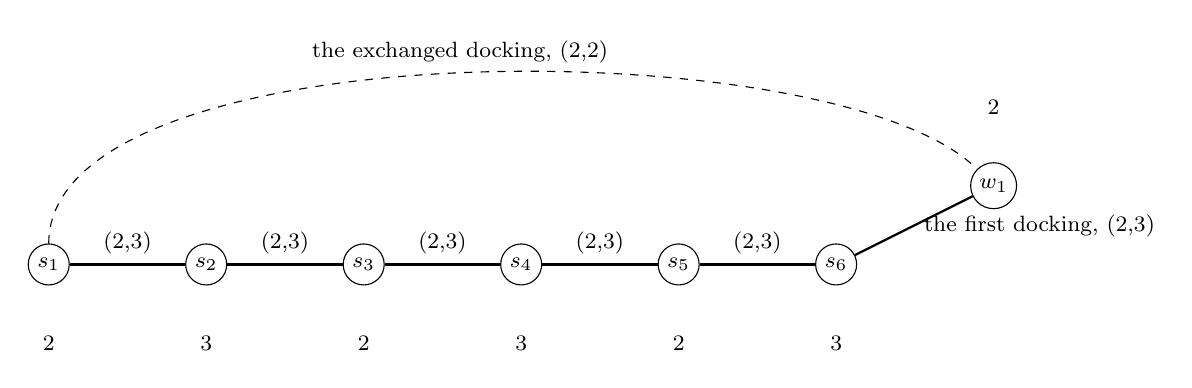
\begin{tikzpicture}[every node/.style={font=\footnotesize}]
\foreach \i/\d in {1/2,2/3,3/2,4/3,5/2,6/3} { \node[circle,draw,inner sep=2pt] (s\i) at (2*\i,0) {$s_{\i}$}; \node at (2*\i,-1) {$\d$}; }
\foreach \i/\j in {1/2,2/3,3/4,4/5,5/6} { \draw[thick] (s\i) -- node[above] {(2,3)} (s\j); }
\node[circle,draw,inner sep=2pt] (w) at (14,1) {$w_1$}; \node at (14,2) {$2$};
\draw[thick] (s6) -- node[right] {the first docking, (2,3)} (w);
\draw[dashed] (s1) .. controls (2,3) and (12,3) .. node[above] {the exchanged docking, (2,2)} (w);
\end{tikzpicture}
\caption{The photon word, six sites of dimensions two and three on five (2,3) links, docking at the electron dock $w_1$. At the first docking its qutrit end $s_6$ meets $w_1$ on a (2,3) pair. At the exchanged docking its qubit end $s_1$ meets $w_1$ on a (2,2) join.}
\end{figure}
\section{The strong reading as a theorem of the rate law}\label{mod:XIV-7-D536664-w-srda}
\begin{chwall}[The strong reading as a theorem of the rate law]\label{box:XIV-7-D536664-w-srda:1}
The three readout rules of the construction part at the junction of the saturated proton, each selecting a different one of the three readings the strong-coupling result prints at the cap register 1036: the gain lemma (the Born count a measure, the readout its root) selects the root reading; the rate law (the rate the prefactor multiplied by the washed square) selects the washed reading, one over 1036; and the readout unit (the normalised trace at the label register) selects the flat reading, one; so no one reading is selected by the rules as a theorem, the strong reading is no theorem of the rate law alone, and the register growth from the first end set 184 to the cap 1036 is a function of the register under every named reading, an open result.
\end{chwall}
\chstanding{open result}
\chdeps{Definitions 1.1 to 1.6 and Table 239.1}{no theorem beyond it at this release}
At one face the three rules would agree at the junction and select one reading as a theorem. At the face this chapter inherits the rules part, each naming its own reading, the parting named with all three objects below. The strong-coupling result and the two running results stand at their own grades, and no reading among the three cells is selected.
\begin{chbridge}
The literature calls the Born count the Born probability, the squared amplitude (exact), the wash the twirl (exact), the washed square the twirled squared amplitude (exact), the register the tensor factors of the common support (nearest), and the object named the strong coupling of quantum chromodynamics running with the scale within a renormalization scheme, its decrease at short distance the asymptotic freedom of Gross, Wilczek and Politzer \cite{Gross1973,Politzer1973}, by name only.
\end{chbridge}
\begin{chproof}[census]
The premises are the Axiom and the six definitions of Section~\ref{mod:FRAMEWORK} (definitions), the records and the Born count of Section~\ref{mod:I-3-records-reads-and-the-born-count-the-gain-lemma} and the read at a register of Section~\ref{mod:I-6-read-at-a-register-the-probe-and-the-measurement} (theorems), and the strong-coupling result and the two running results at their own chapters (read at their grades). Nothing outside that list is used, and the chain from the axiom to this result is three chapters deep.
The set counted is the three readout rules of the construction applied at the junction of the saturated proton, a junction of the genre $(3,3)$, each rule selecting one of the three readings the strong-coupling result prints at the cap register. From the end sets of the junction, by the register at each (none, the center, the far end, both), we obtain the register growth
\begin{equation}
184 \ \to\ 400 \ \to\ 568 \ \to\ 1036 ,
\end{equation}
the first end set at 184 and the cap at 1036, and at the cap the three readings as exact elements,
\begin{equation}
\text{root} = \tfrac{67}{259} + \tfrac{50}{259}\sqrt{3}, \qquad \text{washed} = \tfrac{1}{1036}, \qquad \text{flat} = 1 ,
\end{equation}
with the same three at the center set ($\tfrac{23}{50} + \tfrac{9}{50}\sqrt{3}$, $\tfrac{1}{400}$, $1$) and the far set ($\tfrac{23}{71} + \tfrac{16}{71}\sqrt{3}$, $\tfrac{1}{568}$, $1$). From the gain lemma, by its rule (the Born count a measure, the readout its root), we obtain the selection of the root reading. From the rate law, by its rule (the rate the prefactor multiplied by the washed square), the washed reading, one over 1036, the prefactor beside one over 81 at the one-link first power squared. From the readout unit, by its rule (the normalized trace at the label register), the flat reading, one. The property tested, that the three rules agree at one reading, fails. The rules are re-met at the cap and each names its reading, and they agree at none, which is the first parting element, named with all three objects. From the register under every named reading, by the increments from the center set to the far set and from the far set to the cap, we obtain the growth as a function of the register (the flat increments zero at both steps, the root and the washed moving with the register), so no reading selects a value of the coupling.
The check is by the counter-tests. The junction uncapped at the site product moves the register to 2592 and every reading with it. The dock link read at the cap in place of the junction moves the genre to $(2,3)$ and the register to 319 with the readings at the four roots. The text struck moves every cell. The controls hold, the three readings re-met at the strong-coupling result and the register growth re-met at every end set among them.
The result was reproduced by an independent route, two engines written apart agreeing at every reading, rule and register.
\chcert{3}
\end{chproof}

\section{The hub-step rate as the composite of three cells}\label{mod:IX-2-D541239-w-fchs}
\begin{chwall}[The hub-step rate as the composite of three cells]\label{box:IX-2-D541239-w-fchs:1}
This result is conditional on the parents at their grades, the Fermi open result, the charged-current, pair-ket, three-premises, prefactor, beta-arm, office, every-lepton-office and W-read open results, the composition riding the lowest grade in its chain. The rate over the fifth power of the first power is not the composite of the hub-step amplitude squared, the tick and the W office at any body: at the muon sink the rate $34958/11449$ over the fifth power of $963$ against the composite, the washed square $2831598$ multiplied by the tick $1/927369$ over the W office $\tfrac{2857690241}{3645000} + \tfrac{98}{50625}\sqrt{2}$, parting; at the beta arm the rate over the fifth power of $10773$ against the composite there, parting; at the tau sink no established rate and no established amplitude, undefined; equal at zero of three bodies and at zero of sixty-three points of the grid; the first parting the muon; the composite at the point adopted the rate over the W office, so that the rate over the fifth power is the composite multiplied by the W office over the fifth power of the first power at the muon and at the tau web of the library, the strength as the composite standing at no body.
The first face, the rate over the fifth power equal to the composite at every body, the strength the composite, reads no, equal at zero of three bodies, defined at two of three and at zero of sixty-three points of the grid; the second face, the first parting body named with both cells, reads yes at the muon. Open is the strength of the hub step as a composite of three cells: the rate of a body over the fifth power of its first power and the amplitude squared multiplied by the tick over the W office differ by the W office over the fifth power of the first power, a factor no cell of the three supplies.
\end{chwall}
\chstanding{an open result}
\chdeps{Definitions 1.1 to 1.6 and Theorems 206.1 to 206.4}{no theorem beyond it at this release}
The Fermi open result posed the strength of the weak process as a rate divided by the fifth power of the first power of the decaying body, and this result asks whether that strength is the product of three cells the chain already carries: the hub-step amplitude squared of the charged-current result, the tick cell of the rate results, one over the Born square of the first power, and the W office of the fixed library. At the muon and at the beta arm each cell is an exact number and the composite is an exact element of the field with a root-two part, and it is not the strength: the quotient of the two is the W office over the fifth power of the first power, the same at the muon and at the tau web of the library and different at the beta arm. At the tau sink of the saturation neither a rate nor an amplitude is established, so nothing is compared there. The open result names the muon as the first parting.
\begin{chbridge}
The Fermi constant sets the strength of the weak interaction, the muon lifetime inverse proportional to its square multiplied by the fifth power of the muon mass, and in the electroweak theory the constant is the square of the gauge coupling over the W mass squared \cite{Fermi1934,Weinberg1967}. The correspondence is by name.
\end{chbridge}
\begin{chproof}[exhaustive census with its exact part]
The premises of this derivation are the axiom and the six definitions of chapter~\ref{mod:FRAMEWORK}, the rate as the washed square of the read and the tick unit of the present chapter, a theorem, the prefactor as the tick width of chapter~\ref{mod:IX-3-prefactor-as-the-tick-width}, a theorem, the Fermi constant and the muon decay of the chapter titled The Fermi constant and the muon decay (chapter~\ref{mod:VI-5-fermi-constant-and-the-muon-decay}, among the instruments), a theorem, the charged and neutral currents of the chapter titled The charged and neutral currents (chapter~\ref{mod:VI-4-charged-and-neutral-currents}, among the instruments), a theorem, and the Higgs and carrier offices at their sinks of chapter~\ref{mod:VI-10-higgs-the-closed-hub-read-its-rows-its-mass-and-its-exponent}, a theorem. The chain of premises runs back to the axiom through those chapters, and the longest such chain in this compendium is twelve chapters long.
\textit{The exact part.} At the muon sink the first power is $963$, the rank $107$ by the dressing $9$, re-met at seven of seven cells, the rate of the Fermi open result is $34958/11449$, the hub-step amplitude squared is the washed square of the forward readouts of the charged-current result over its twenty-nine edges, $2831598$, the tick is one over the Born square of the first power, $1/927369$, and the W office of the library word is $\Omega_{W} = \tfrac{2857690241}{3645000} + \tfrac{98}{50625}\sqrt{2}$. The strength and the composite read
\begin{equation} \frac{34958/11449}{963^{5}} \qquad\text{against}\qquad \frac{2831598\cdot\tfrac{1}{927369}}{\Omega_{W}}, \qquad \frac{\text{strength}}{\text{composite}} = \frac{\Omega_{W}}{963^{5}}, \end{equation}
the two parting at the muon, the composite an element with a root-two part; the quotient equals the W office over the fifth power of the first power at the muon and at the tau web of the library, $3969$ at the first power with the amplitude squared $19597707$ over twenty-two edges and the tick $1/15752961$, and parts at the beta arm, the first power $10773$, the amplitude squared $153966987$ over nineteen edges and the tick $1/116057529$, where the dock-class arm cell of the Fermi open result stands against the hub-class amplitude. At the tau sink the first power is $4185$ and the tick $1/17514225$, but no rate and no amplitude are established, so the composite is undefined there. The figure draws the hub step at the muon sink.
\textit{The census.} By exhaustive enumeration of the sixty-three points of the grid, two definitions of the first power by three ticks by five readings of the W office by two powers with the charged-current rate reading and the unwashed and count amplitudes beside, at the three bodies: the property tested is equality of the rate over the fifth power with the composite; the count is equal at zero of three bodies at the point adopted and at zero of sixty-three points, the composite at the point adopted equal to the rate over the W office by construction at three of three established bodies. The smallest case is the muon worked above.
\textit{The check.} The counter-tests alter the construction singly and read what moves. Striking the exponent to one moves the strength at the muon. Reading the muon amplitude at its unwashed square moves the composite. Reading the W office at the dock face moves the office with the strength holding. Composing the rates, every established rate replaced by the composite multiplied by the fifth power, moves the first parting from the muon to the tau sink. Striking the gate unmeets it. Each alteration moves the cells it names, five of five. The result was reproduced by an independent route, two engines built apart, the exact-fraction route against the second route, equal at every cell, with the sixteen controls the same.
\chcert{63}
\begin{figure}[h]\centering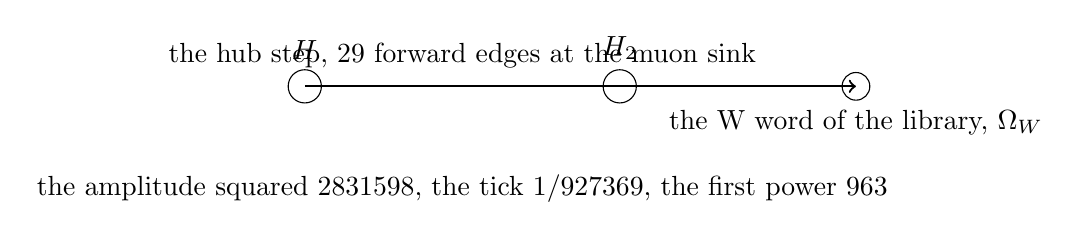
\begin{tikzpicture}[scale=1]
\filldraw[fill=white] (0,0) circle (6pt) node[above=6pt] {$H$}; \filldraw[fill=white] (4,0) circle (6pt) node[above=6pt] {$H_2$};
\draw[thick] (0,0) -- (4,0);
\node at (2,0) [above=3pt] {the hub step, 29 forward edges at the muon sink};
\filldraw[fill=white] (7,0) circle (5pt) node[below=5pt] {the W word of the library, $\Omega_W$};
\draw[thick,->] (4,0) -- (7,0);
\node at (2,-1) [below] {the amplitude squared $2831598$, the tick $1/927369$, the first power $963$};
\end{tikzpicture}\caption{The three cells of the composite at the muon sink: the hub step between its two hubs with its washed square, the tick from the first power, and the W office of the library word.}\end{figure}
\end{chproof}
\section{The number and the vacuum term in tick units}\label{mod:IX-2-D543234-w-nmvt}
\begin{chwall}[The number and the vacuum term in tick units]\label{box:IX-2-D543234-w-nmvt:1}
Of the three elements of the item the area coefficient parts first: the cut register of the horizon web is one register at every rung of the fixed cut, 236196 at every crossing link and 6561 at the dark wires, the entropy two log two plus ten log three and eight log three, while the hidden records grow by three per qubit rung, so the ratio of the hidden count to the log reads three over the log at the rungs zero and one and parts at the rung two, six over the same log, and at the moving cut the register moves at the rung one; the coupling element at the electron, the two-point element per unit office multiplied by the office squared, and the vacuum term, the closure constant two over the whole 36 to the sixth, per unit of the measure of the cut and per the (2,2) depth, are exact elements printed; both faces are printed, neither is selected, and no observed value is used.
The first face, the three elements exact and printed with the area coefficient fixed at every rung, reads no, the coefficient parting at the rung two at the fixed interface and at the rung one at the moving interface at every series; the second face, the first of the three not exact or not fixed named with its first parting, reads yes at the area coefficient at the open-end face at the fixed interface at the rung two, the hidden records six against three over the one register. Open is the area coefficient: the cut register of the horizon stays one register while the hidden records grow, so no constant of the horizon web relates the hidden count to the entropy of the cut.
\end{chwall}
\chstanding{an open result}
\chdeps{Definitions 1.1 to 1.6 and Theorems 206.1 to 206.4}{no theorem beyond it at this release}
Three numbers are asked of the horizon web in the units of the tick. The first is an area coefficient, the proportionality between the hidden records across the horizon and the entropy of its cut, the logarithm of the cut register; but the cut of the horizon web is the same three links at every rung, two dark (3,3) wires and the (2,3) tether, so its register and its entropy are one number at every rung, while the hidden records grow by three per qubit rung, and the ratio doubles at the second rung. The second is the coupling at the electron, the (2,2) two-point element per unit office multiplied by the square of the electron office, an exact element of the field. The third is the vacuum term, the closure constant of the counting face, two over the whole of the read genre to the depth exponent six, per unit of the measure of the cut, an exact rational at both readings. The open result names the first as the parting and prints the other two.
\begin{chbridge}
The entropy of a black hole is proportional to the area of its horizon with a coefficient of one quarter in Planck units, the gravitational coupling sets that unit, and the cosmological constant is the vacuum energy density of the field equations \cite{Bekenstein1973,Wald1984}. The correspondence is by name.
\end{chbridge}
\begin{chproof}[finite computation with its exact part]
The premises of this derivation are the axiom and the six definitions of chapter~\ref{mod:FRAMEWORK}, the rate as the washed square of the read and the tick unit of the present chapter, a theorem, the horizon at every rung of chapter~\ref{mod:X-3-horizon-at-every-rung-and-the-horizon-web-as-a-seeded-saturation}, a theorem, the cosmological term at the depth exponent of chapter~\ref{mod:X-6-cosmological-term-at-the-depth-exponent}, a theorem, and the register tower and the metric of chapter~\ref{mod:X-5-register-tower-and-the-metric}, a theorem. The chain of premises runs back to the axiom through those chapters, and the longest such chain in this compendium is twelve chapters long.
\textit{The object.} The horizon web at the attachment site of the horizon result is cut at a fixed interface by three links at every rung, two dark (3,3) wires and the (2,3) tether, whose wholes are 81, 81 and 36, with the crossing census over the genres (2,2), (2,3), (2,4), (3,3), (3,4) and (4,4) reading zero, one, zero, two, zero and zero at every rung and reading, the counted (2,2) crossings zero at 28 of 28 cells. The figure draws the cut.
\textit{The procedure.} At every reading of the attachment site, the open-end face and the docking-lemma face with the closure-site face beside, and every rung zero to six, take the cut register as the product of the wholes of the crossing links and its entropy as the formal logarithm, the exponent vector over the primes. Read the hidden records of the area-law result at each rung and form their ratio to the entropy. Take the (2,2) two-point element of the two-point result per unit office, the tick of one link, multiply by the electron office squared for the coupling element. Take the closure term of the counting face as the curvature-coefficient result carries it and divide by the measure of the cut per the (2,2) depth for the vacuum term. Decide each element exact and the coefficient fixed across the rungs.
\textit{The smallest instance.} At the fixed interface the register and its entropy are
\begin{equation} \adjustbox{max width=\dimexpr\linewidth-3em\relax}{$\displaystyle \begin{gathered} R_{\mathrm{cut}} = 81\cdot 81\cdot 36 = 236196 = 2^{2}\cdot 3^{10}, \\ S_{\mathrm{cut}} = 2\log 2 + 10\log 3, \\ R_{\mathrm{dark}} = 6561, \quad S_{\mathrm{dark}} = 8\log 3, \end{gathered}$} \end{equation}
one register at every rung, while the hidden records at the open-end face read 3, 3, 6, 6, 9, 9 and 12 at the rungs zero to six and 3, 3, 6, 9, 12, 15 and 18 at the docking order, so the coefficient reads
\begin{equation} \frac{3}{2\log 2 + 10\log 3} \ \text{at the rungs } 0 \text{ and } 1, \qquad \frac{6}{2\log 2 + 10\log 3} \ \text{at the rung } 2, \end{equation}
the first parting at the rung two, and at the moving interface the register itself moves at the rung one. The coupling element at the electron is the two-point element $\tfrac{5}{384} + \tfrac{5}{384}\sqrt{2}$, the register sum $30 + 30\sqrt{2}$ over 2304, per unit office one, multiplied by the square of the electron office, an element whose rational coordinate carries sixteen digits, the product an exact element of the field. The vacuum term is the closure term
\begin{equation} \Lambda = \frac{2}{36^{6}} = \frac{1}{1088391168}, \end{equation}
equal to the curvature-coefficient result, and per unit of the measure of the fixed cut it is that term over $2\log 2 + 10\log 3$ at the formal reading and over the register at the count reading, exact at both; the (3,3) vacuum register 6561 and the closure constant over that tower, two over 6561, stand beside.
\textit{The check.} The counter-tests alter the construction singly and read what moves. Striking the tether from the census moves the register from 236196 to 6561 at 513 cells. Reading the (3,3) crossing count in place of the whole moves the register to eight and the entropy to three log two. Replacing the electron office by the muon office moves the coupling element to a four-coordinate element. Shifting the hidden records one rung moves the first parting to the rung one. Striking the text unmeets the gate. Each alteration moves the cells it names, five of five. The result was reproduced by an independent route, two engines built apart, the exact-fraction route against the second route, equal at every cell, with the thirteen controls the same.
\chcert{28}
\begin{figure}[h]\centering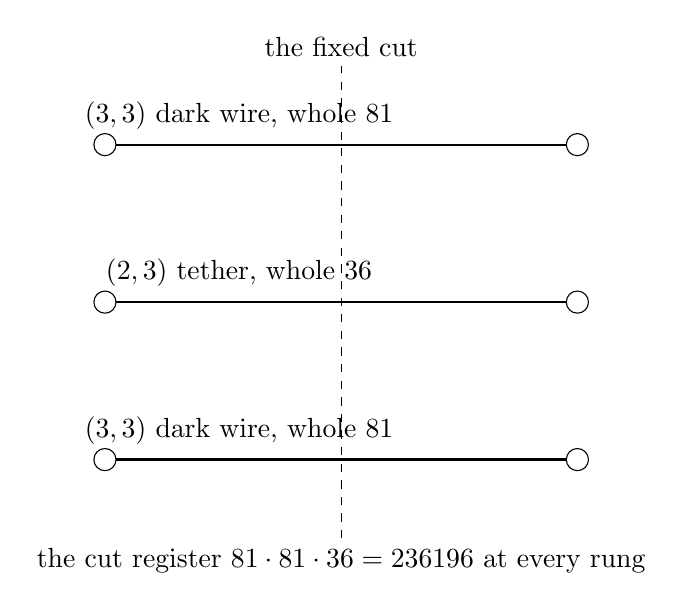
\begin{tikzpicture}[scale=1]
\draw[dashed] (3,-3) -- (3,3); \node at (3,3) [above] {the fixed cut};
\foreach \y/\l/\w in {2/{$(3,3)$ dark wire, whole $81$}/81, 0/{$(2,3)$ tether, whole $36$}/36, -2/{$(3,3)$ dark wire, whole $81$}/81} {\draw[thick] (0,\y) -- (6,\y); \filldraw[fill=white] (0,\y) circle (4pt); \filldraw[fill=white] (6,\y) circle (4pt); \node at (1,\y) [above=2pt, xshift=20pt] {\l};}
\node at (3,-3) [below] {the cut register $81\cdot 81\cdot 36 = 236196$ at every rung};
\end{tikzpicture}\caption{The cut of the horizon web at its fixed interface: two dark (3,3) wires and the (2,3) tether, whose register is one number at every rung while the hidden records grow.}\end{figure}
\end{chproof}
\par\medskip\noindent{\itshape The square read, the next chapter reads the factor that multiplies it.}\label{narr:close:9-2}\par
\section{The prefactor as the tick width}\label{mod:IX-3-prefactor-as-the-tick-width}
\chdesig{12-3}{9-3}{IX-3-prefactor-as-the-tick-width}{IX-3-prefactor-as-the-tick-width}
\label{narr:open:9-3}Theorem~210.2 reads the prefactor as the tick width, with the prefactor from the record office width, Open result~210.1, open beside it.
\begin{chwall}[Prefactor from record office width]\label{box:IX-3-prefactor-as-the-tick-width:1}
The prefactor read as the tick width multiplied by the office register is not an output of the derived rate cells: at the one-link read the tick width of the electron multiplied by the pinned register parts from the Compton objects at the first cell, at the hub-transfer read the width of the muon multiplied by the W-word register parts from the coherent-release rate, and the prefactor the cells imply is the inverse Born square of the measuring body, a candidate grid of widths, registers and squares matching the cells at the prefactor one alone.
\end{chwall}
\chstanding{open result}
\chdeps{Definitions 1.1 to 1.6, Theorems 28.1 and 28.2, Open results 28.3 and 28.4 and Theorem 28.5 and Theorems 206.1 to 206.4}{Theorems 211.1 and 211.2}
\begin{chconditional}[The prefactor as the tick width]\label{box:IX-3-prefactor-as-the-tick-width:2}
Conditional on the results it rests on, among them prefactor from record office width, rate as the washed square of the read, coherent release as the unwashed square at the joined web, the unstable row correction as the open move readout and decay graph as the census graph at the stop condition, each at its own standing. At every rate-form cell of the two rate results the prefactor is the inverse Born square at the office: at the Compton objects and at the coherent-release rates over the Born square of the joined web, the cell over the square of the same read at its own wash equals one over the office register squared, the office register being the first power of the measuring body at the hub reading, the dock-struck first power at the dock reading, the unit at the unit reading and the first power of the joined web at the coherent release.
\end{chconditional}
\chstanding{conditional theorem}
\chdeps{Definitions 1.1 to 1.6, Theorems 28.1 and 28.2, Open results 28.3 and 28.4 and Theorem 28.5 and Theorems 206.1 to 206.4}{Theorems 211.1 and 211.2}
The offices are listed at the hub, dock and unit readings and at the joined web at every copy count, the Born square is constructed as the office register squared, every rate-form cell is divided by the square of the same read at its own wash and compared with the inverse office square, and the prefactor is typed as the inverse office at every cell and as the inverse one-link register, the inverse W-word register or the inverse dock office square at none. The theorem rests on the rate law, the coherent release, the tick width and the wash at one act, and the parted reading, the prefactor as the tick width multiplied by the office register, is recorded beside it. It is the reading the theorem re-meets at its parting, every figure of it an output of the derived tables.
\begin{chbridge}
In the standard account the rate of the golden rule carries a prefactor set by the normalization of the states and the phase-space measure, so that a width is a squared matrix element multiplied by a density of final states \cite{Dirac1927,Fermi1934}. The correspondence is by name.
\end{chbridge}
\begin{chproof}[exhaustive census]
\textit{The premises.} The axiom and the six definitions of Section~\ref{mod:FRAMEWORK}, definitions. The read at a register of Section~\ref{mod:I-6-read-at-a-register-the-probe-and-the-measurement}, a theorem. The rate as the washed square of Section~\ref{mod:IX-2-rate-as-the-washed-square-of-the-read-and-the-tick-unit}, a theorem. The coherent release, the tick as the unit of the rate and the Born squares as the first powers squared, theorems. The prefactor reading of the preceding chapter, an open result consumed at its registers. The chain from the axiom to this result is seven chapters deep.

\textit{The census.} The set counted is the rate-form cells of the two rate results, the 24 Compton objects of the rate law (three Born readings, four census readings, two dockings) and the 36 coherent-release rates over the Born square of the joined web (three joins, four copy counts, the washed and the two unwashed matchings), 60 cells in all, with 44 square cells and 12 pair-creation objects beside. At each cell the office register is the first power of the measuring body at the reading of the cell, $201$ at the hub reading (the Born square $40\,401$), $67$ at the dock reading ($4489$), one at the unit reading, and at the coherent release the first power of the joined web, $963$ at one copy (the muon first power) and $17\,334$, $234\,009$ and $2\,808\,108$ at two, three and four copies, the integer roots of the Born squares of the joined web, perfect squares at 12 of 12. The property tested at each cell is whether the cell over the square of the same read at its own wash equals one over the office register squared,
\begin{equation}
\frac{\text{cell}}{(\text{the read})^{2}}=\frac{1}{\text{office}^{2}} ,
\end{equation}
at the Compton object at the first docking $5/40\,401$ the prefactor $1/40\,401$ against $1/201^{2}$, at the dock reading $1/4489$, at the unit reading one, at the coherent release at one copy $1/927\,369$ against $1/963^{2}$. The count is 60 of 60 equal, at the derived offices 33 of 33 and at the root offices 27 of 27, the prefactor typed the inverse office at 60, one at 0 and other at 0, the first parting none. The smallest case is the unit reading, where the office is one and the prefactor one, checked by hand. Beside, at the washed reading of the preceding prefactor result the count is 36 of 60, the 24 unwashed cells carrying the ratio of the unwashed to the washed square, $1+\tfrac{2}{3}\sqrt{2}$ at one copy and $2+\tfrac{4}{3}\sqrt{2}$, $3+2\sqrt{2}$ and $4+\tfrac{8}{3}\sqrt{2}$ at two, three and four copies at the one-read matching, outside the rationals at 24 of 24. Against the one-link register, the W-word register and the dock office square the count is 0 of 60 each.

\textit{The check.} Rotating the office readings one step moves the count from 60 to 36 of 60. Reading the unwashed cells over the washed square moves it to 36. Replacing the office by the one-link register moves it to zero. Taking the Born square of the joined web at one copy everywhere moves it to 33. The result was reproduced by an independent route, two engines of different construction agreeing at every cell at both runs, with the Compton objects at 24 of 24, the coherent-release rates at 36 of 36 and the implied prefactors of the preceding result at 104 of 104 as the controls.
\chcert{3316}
\end{chproof}
\par\medskip\noindent{\itshape Rate and prefactor together give lifetimes and branching, read in the next chapter.}\label{narr:close:9-3}\par
\section{The imbalance readout, lifetimes and branching}\label{mod:IX-4-imbalance-readout-lifetimes-and-branching}
\chdesig{12-4}{9-4}{IX-4-imbalance-readout-lifetimes-and-branching}{IX-4-D543346-w-lftd}
\label{narr:open:9-4}Theorem~211.1 reads the imbalance readout with the lifetimes and the branching, and Theorem~211.2 reads the baryon asymmetry as the sign of the imbalance at the universe web.
\begin{chconditional}[The imbalance readout, lifetimes and branching]\label{box:IX-4-imbalance-readout-lifetimes-and-branching:1}
Conditional on the results it rests on, among them the decay rate as the imbalance readout, the prefactor as the inverse Born square at the office, rate as the washed square of the read, first power as the act readout sum, decay graph as the census graph at the stop condition and the unstable row correction as the open move readout, each at its own standing. The hierarchy of the three kinds of readout by structure alone is an output of the registers: the washed squares over the registers order the three kinds strictly, the (2,3) kind above the hub-leg kind at (2,4) above the (3,3) kind, and the same at every non-sink because a register is a constant of the genre and not of the body; the count clause of the rate law, the washed squares multiplied by the prefactor and the forward-edge count, overturns the structural order wherever a dock edge stands beside the hub edges, first at the one-dock electron body, a display of the rate law and no parting of the registers.
\end{chconditional}
\chstanding{conditional theorem}
\chdeps{Definitions 1.1 to 1.6, Theorems 9.1 to 9.7 and Open result 9.8, Theorems 206.1 to 206.4 and Open result 210.1 and Theorem 210.2}{Table 205.1 and Open result 212.1}
\begin{chconditional}[The baryon asymmetry as the sign of the imbalance at the universe web]\label{box:IX-4-imbalance-readout-lifetimes-and-branching:2}
Conditional on the results it rests on, each at its own standing. The sign census of the forward edges of the universe web carries a definite excess: the recorded forward edges of the horizon web at its first wave are every one signed at the register count, the three sign readings agree at every edge, the excess runs toward lowering, the hub, dock and core kinds lowering and the triangle pairings raising, the letters at the ends of the removed links balance at every edge so that the asymmetry sits at the register direction, and the share of the total readout is an exact rational keyed to no observed value, under the bound of the depth result.
\end{chconditional}
\chstanding{conditional theorem}
\chdeps{Definitions 1.1 to 1.6, Theorems 9.1 to 9.7 and Open result 9.8, Theorems 206.1 to 206.4 and Open result 210.1 and Theorem 210.2}{Table 205.1 and Open result 212.1}
The three kinds of readout are listed at their registers, the washed squares over the registers ordered, the order checked at every non-sink restricted to the kinds present, and the count clause printed beside as a display of the rate law. The forward edges of the universe web are signed at the register count at the depth result's reading, the three sign readings compared, and the census summed by kind with the end letters balanced, under the bound of the depth result. The branching ratios of the previous chapter are the shares of the washed squares at the multi-channel non-sinks, summing to one by body alone, and the lifetime of a non-sink is the inverse of its total width with the tick as its unit. What stands open is not a question of this chapter. The hierarchy rests on the open questions among its premises, and the baryon asymmetry holds under the bound of the depth result, beyond which nothing is claimed.
\begin{chbridge}
In the standard account the lifetimes of the unstable particles span many orders of magnitude and sort by the interaction that drives the decay, the strong decays the fastest and the weak the slowest, the hierarchy read off the couplings and the phase space of the golden rule \cite{Fermi1934,WeisskopfWigner1930}, and the branching ratio of a channel is its partial width over the total width. The correspondence is by name.
\end{chbridge}
\begin{chproof}[finite computation]
\textit{The premises.} The axiom and the six definitions of Section~\ref{mod:FRAMEWORK}, definitions. The link and its six genres of Section~\ref{mod:I-2-link-and-its-six-genres}, definitions. The rate as the washed square and the prefactor of Sections~\ref{mod:IX-2-rate-as-the-washed-square-of-the-read-and-the-tick-unit} and \ref{mod:IX-3-prefactor-as-the-tick-width}, theorems. The gain lemma, the six-genre result, the tick width, the gluon closed read and the first-power result, theorems. The one-genre, decay-graph, unstable-row, strong-coupling, seed and saturation questions, open results read as they stand. The chain from the axiom to this result is eight chapters deep.

\textit{The procedure.} The input objects are the six genres with their coherent sums and Born faces re-derived from the sectors of the gain lemma, equal to the derived cells at 6 of 6,
\begin{equation} \adjustbox{max width=\dimexpr\linewidth-3em\relax}{$\displaystyle (2,3):\ 79+48\sqrt{2}+42\sqrt{3}+3\sqrt{6}\ \text{at the Born face }319;\quad (2,4):\ 450+96\sqrt{2}\ \text{at }906;\quad (3,3):\ 268+200\sqrt{3}\ \text{at }1036,$} \end{equation}
with $(3,4)$ at $2053$, $(2,2)$ at $96$ and $(4,4)$ at $5100$. The enumeration rule runs as follows. At each genre the register adopted is the cut register to the first non-vanishing order multiplied by the whole register to the three less that order ($31\,104$ at $(2,3)$, $129\,600$ at $(2,4)$, $331\,776$ at $(3,3)$), and the washed square over the register is the Born face over the register squared,
\begin{equation}
\frac{319}{967\,458\,816}\ \text{at }(2,3),\qquad \frac{151}{2\,799\,360\,000}\ \text{at the hub-leg kind }(2,4),\qquad \frac{259}{27\,518\,828\,544}\ \text{at }(3,3).
\end{equation}
The test applied is the order of the three readouts, taken at every ordered pair as an exact ratio. The aggregation is the ordering at every non-sink restricted to the kinds present. The ratios at the reading adopted are
\begin{equation}
\frac{(2,3)}{\text{hub-leg}}=\frac{199\,375}{32\,616},\qquad \frac{(2,3)}{(3,3)}=\frac{81\,664}{2331},\qquad \frac{\text{hub-leg}}{(3,3)}=\frac{927\,744}{161\,875},
\end{equation}
each the Born-face ratio multiplied by the squared register ratio, within two powers of ten and within one power of the whole register thirty-six, so the forced ordering is strict, the $(2,3)$ kind above the hub-leg kind above the $(3,3)$ kind. The smallest instance is one ratio, $319/906$ multiplied by $(25/6)^{2}$, checked by hand.

\textit{The thirteen non-sinks.} The non-sinks of the decay graph at the stop reading are thirteen of the seventy-four primary webs, every forward edge a hub-step move at 13 of 13, so every non-sink is assigned to the hub-leg kind at the $(2,4)$ genre. The ordering by the washed squares over the registers is the same at every one because a register is a constant of the genre and not of the body, equal at 13 of 13 restricted to the kinds present, the first parting none, which is the statement. The ratios are exact at 108 of 108 over the eighteen readings. The count clause beside, the prefactor multiplied by the forward-edge count multiplied by the washed square, equals the forced ordering at 7 of 13 and parts at 6 of 13, first at the one-dock electron body, where twenty hub-leg edges stand beside one dock edge at a per-edge ratio of about six. Every parting non-sink carries a dock edge, the parting a display of the rate law and no parting of the registers.

\textit{The check.} The order the preceding reading named as a hypothesis, the hub-leg kind below the $(2,3)$ kind below the $(3,3)$ kind, is met at 0 of 18 readings. The alterations of the register, the wash and the kind assignment each move the ordering they name. The result was reproduced by an independent route, two engines of different construction agreeing at every cell at both runs, with the gain-lemma sectors, the six-genre registers and the one-genre parting as the controls.
\chcert{108}
\end{chproof}
\begin{figure}[htbp]\centering
{\scriptsize\setlength{\tabcolsep}{3pt}\begin{adjustbox}{max width=\linewidth}\begin{tabular}{p{22mm}p{12mm}p{34mm}rrp{40mm}}
the class & the genre & the sectors & the Born face & the register & the washed square over the register \\ \hline
the (2,3) class & (2,3) & odd 79, mixed-even 48, same-even 42, closure 3 & 319 & 31104 & 319/967458816 \\
the hub-leg class & (2,4) & odd 198, mixed-even 90, same-even 126, closure 3 & 906 & 129600 & 151/2799360000 \\
the (3,3) class & (3,3) & odd 184, mixed-even 128, same-even 72, closure 28 & 1036 & 331776 & 259/27518828544 \\
\end{tabular}\end{adjustbox}}
\par\smallskip
{\scriptsize\begin{adjustbox}{max width=\linewidth}\begin{tabular}{p{50mm}rp{80mm}}
the ratio of two classes & the ratio & the factor \\ \hline
the (2,3) class to the hub-leg class & 199375/32616 & born 319 over 906 multiplied by the register ratio 25/6 squared \\
the (2,3) class to the (3,3) class & 81664/2331 & born 319 over 1036 multiplied by the register ratio 32/3 squared \\
the hub-leg class to the (3,3) class & 927744/161875 & born 906 over 1036 multiplied by the register ratio 64/25 squared \\
\end{tabular}\end{adjustbox}}
\par\smallskip
{\footnotesize the forced ordering at the reading of record: the (2,3) class $>$ the hub-leg class $>$ the (3,3) class}
\par\smallskip
{\scriptsize\setlength{\tabcolsep}{3pt}\begin{adjustbox}{max width=\linewidth}\begin{tabular}{p{44mm}rp{52mm}p{24mm}}
the non-sink & first power & the ordering at the cells the decay rows print & against the forced ordering \\ \hline
the one-dock electron body & 201 & the hub-leg class $>$ the (2,3) class & parts \\
the muon body & 963 & the hub-leg class $>$ the (2,3) class & parts \\
the two-dock muon word & 963 & the hub-leg class $>$ the (2,3) class & parts \\
the tau body & 3969 & the hub-leg class & equal \\
the two-dock tau word & 3969 & the hub-leg class & equal \\
the K-rep web K0 & 48 & the hub-leg class $>$ the (2,3) class & parts \\
the K-rep web K1 & 72 & the hub-leg class $>$ the (2,3) class & parts \\
the K-rep web K2 & 1248 & the hub-leg class $>$ the (3,3) class & equal \\
the closed tau & 4077 & the hub-leg class & equal \\
the gluon body & 27 & the hub-leg class $>$ the (3,3) class & equal \\
the Higgs body & 16 & the hub-leg class & equal \\
the seed S & 219 & the hub-leg class $>$ the (3,3) class $>$ the (2,3) class & parts \\
the seed R & 4 & the hub-leg class & equal \\
\end{tabular}\end{adjustbox}}
\caption{The lifetime hierarchy as the class readouts. The three classes of the forward edges of a non-sink, the (2,3) class, the hub-leg class at the (2,4) genre and the (3,3) class, each with its sectors, its Born face, its register at the first non-vanishing order and its washed square over the register at the reading of record; the ratio of two class cells is the Born-face ratio multiplied by the register ratio squared, and the ordering of the three classes is forced by the registers, the (2,3) class $>$ the hub-leg class $>$ the (3,3) class. At the cells the decay results print for the 13 non-sinks the ordering restricted to the classes present meets the forced ordering at 7 of 13, the first parting the one-dock electron body; at the universal cells it meets it at 13 of 13 (the lifetimes of the literature are the readouts by name).}\label{fig:lifetime-hierarchy}
\end{figure}
\section{The lifetimes as termination depths}\label{mod:IX-4-D543346-w-lftd}
\begin{chwall}[The lifetimes as termination depths]\label{box:IX-4-D543346-w-lftd:1}
The rates the decay results print are not the termination depths at the couplings, the first decay parting the one-dock electron body: every one of the twenty-five unstable configurations of the three decay results carries its sink at the terminal web of the longest chain of hub-step inverse edges, the muon web of the library to the two-dock electron web at the depth one, the tau web through the muon web at two, the closed tau at two, the bottom-docked body to the up body at three, fourteen of twenty-five at their sink already at the depth zero, the hub ladder equal to the depth at twenty-four of twenty-four with both anatomies; the coupling at the (2,4) cells of the path is the six-dressings element $\tfrac{5}{2048} + \tfrac{1}{1920}\sqrt{2}$ at both spellings and the depth per unit coupling an exact element at twenty-five of twenty-five; the thirty-five established rate cells equal the depth per unit coupling at two of thirty-five, the proton sink and the neutron twin at the board cell zero and the depth zero, and part at thirty-three of thirty-five, the first parting the one-dock electron body at the imbalance-readout result, $24028/4489$ against zero at the depth zero; the Fermi-strength open result re-posed at the depth count is re-named, the muon $34958/11025387$ against the tau web $2987/37822859361$ and the beta arm $36/17689$, equal at zero of three pairs, and the composite open result re-posed is re-named, parting at three of three bodies; both faces are printed, neither is selected, and no observed value is used.
The first face, the rates the termination depths at the couplings at every established decay, reads no, the configurations listed with their sinks at twenty-five of twenty-five and the depths exact at twenty-five of twenty-five but the rate cells equal to the depth per unit coupling at two of thirty-five alone; the second face, the first decay parting named, reads yes at the one-dock electron body. Open is the rate as a depth count: the rates are washed squares of the forward readouts over the Born square of the first power, exact rationals, while the depth per unit coupling is an integer count multiplied by the inverse of a ring element carrying root two, so the two coincide at the zero cells alone.
\end{chwall}
\chstanding{an open result}
\chdeps{Definitions 1.1 to 1.6 and Theorems 211.1 and 211.2}{no theorem beyond it at this release}
A decaying configuration reaches its sink along a chain of hub-step inverse edges, each lowering the hub count by one, and the length of that chain is its termination depth; the muon web is one step from the electron web and the tau web two, the bottom-docked body three steps from the up body, and fourteen of the twenty-five configurations are sinks already. The question is whether the rates the decay results print are these depths measured per unit of the (2,4) coupling. They are not: a rate is a washed square over the Born square of a first power, a rational number, whereas a depth per unit coupling carries root two, and the two agree only where both are zero, at the two stable configurations. The first configuration in the frozen order, the one-dock electron body, has a nonzero rate and no terminating path within the established webs, so it parts first, and the two foregoing open results re-posed as depth counts are re-named rather than met.
\begin{chbridge}
The lifetime of an unstable particle is the inverse of its total decay width, computed in the Standard Model from the matrix elements of its decay channels and the phase space available, the muon lifetime scaling as the inverse fifth power of its mass multiplied by the Fermi constant squared \cite{Fermi1934,Peskin1995}. The correspondence is by name.
\end{chbridge}
\begin{chproof}[finite computation with its exact part]
The premises of this derivation are the axiom and the six definitions of chapter~\ref{mod:FRAMEWORK}, the imbalance readout, lifetimes and branching of the present chapter, a theorem, the decay as the forward edge of a non-sink of chapter~\ref{mod:IX-1-decay-as-the-forward-edge-of-a-non-sink-the-move-graph-of-the-hub-step}, a theorem, the rate as the washed square of the read of chapter~\ref{mod:IX-2-rate-as-the-washed-square-of-the-read-and-the-tick-unit}, a theorem, the depth, the growth order and the termination wave of chapter~\ref{mod:X-4-depth-the-growth-order-and-the-termination-wave}, a theorem, and the six dressings at the six genres of chapter~\ref{mod:VIII-1-mass-unit-and-the-first-power}, an open result. The chain of premises runs back to the axiom through those chapters, and the longest such chain in this compendium is twelve chapters long.
\textit{The objects.} The twenty-five unstable configurations are the thirteen non-sinks of the imbalance-readout result at its sink reading in its table order, the three sinks of the decay-board map carrying a cell not among them, and the nine sinks of the charged-current result not among them, each with its hub count, dressing and first power by locator, and the decay graph is the edges table of the decay-graph result. The figure draws the terminating path of the tau web.
\textit{The procedure.} For each configuration follow the hub-step inverse edges at the targets alone, a web beyond the established reached never, and take the terminal web of the longest such chain as its sink and the serial count of ticks along it at one move one tick, as the rate law counts a move, as its termination depth. Read the coupling at the (2,4) cells of the path as the six-dressings element of that genre at both spellings. Divide the depth by the coupling for the depth per unit coupling. Parse each of the thirty-five established rate cells of the four results as an exact element and compare it with the depth per unit coupling at both spellings.
\textit{The smallest instance.} The depths at the reading adopted are zero at the docked electron, one at the muon web and the two-dock muon word, two at the tau web and the two-dock tau word, zero at the three representative webs, two at the closed tau, zero at the gluon and Higgs bodies and the two seeds, zero at the two-dock electron, the proton sink and the neutron twin, zero at the electron-face sink and the proton seed, one at the star-face sink, zero at the up-docked body, one at the down-docked and charm-docked bodies, two at the strange-docked and top-docked bodies and three at the bottom-docked body, an exact count at twenty-five of twenty-five, with the hub ladder equal to the depth at twenty-four of twenty-four. The coupling and the depth per unit coupling at the muon web read
\begin{equation} c_{24} = \frac{450 + 96\sqrt{2}}{184320} = \frac{5}{2048} + \frac{1}{1920}\sqrt{2}, \qquad \frac{1}{c_{24}} = \frac{2304000}{5113} - \frac{491520}{5113}\sqrt{2}, \end{equation}
against the rate $34958/11449$ of the imbalance-readout result, parting; at the one-dock electron body the rate is $24028/4489$ against the depth per unit coupling zero, its five hub-step inverse edges every one reaching a web beyond the established so that its terminating path is empty and its sink itself, the first parting in the frozen order; at the proton sink and the neutron twin the board cell zero equals the depth zero, the two equal cells of thirty-five. The Fermi-strength open result re-posed at the depth count reads $34958/11025387$ at the muon, $2987/37822859361$ at the tau web and $36/17689$ at the beta arm, equal at zero of three pairs, re-named, and the composite open result re-posed parts at three of three bodies, re-named.
\textit{The check.} The counter-tests alter the construction singly and read what moves. Striking one tick of every terminating path moves the muon web and the two-dock muon word to the depth zero and the tau web to one. Striking the coupling to one reads the depth itself. Reading the (2,3) path in place of the (2,4) moves the coupling to the (2,3) element. Reading every configuration at its sink already moves every depth to zero. Striking the text unmeets the gate. Each alteration moves the cells it names, five of five, the face and the first parting unmoved at the four strikes. The result was reproduced by an independent route, two engines built apart, the exact-fraction route against the second route, equal at every cell, with the fourteen controls the same.
\chcert{25}
\begin{figure}[h]\centering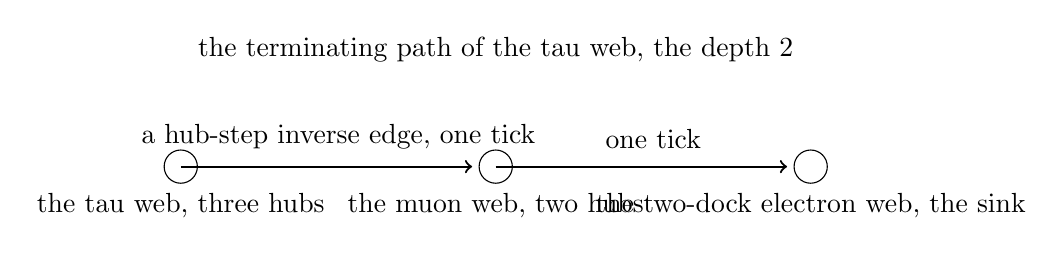
\begin{tikzpicture}[scale=1]
\filldraw[fill=white] (0,0) circle (6pt) node[below=6pt] {the tau web, three hubs};
\filldraw[fill=white] (4,0) circle (6pt) node[below=6pt] {the muon web, two hubs};
\filldraw[fill=white] (8,0) circle (6pt) node[below=6pt] {the two-dock electron web, the sink};
\draw[thick,->] (0,0) -- (37mm,0); \draw[thick,->] (4,0) -- (77mm,0);
\node at (2,0) [above=3pt] {a hub-step inverse edge, one tick}; \node at (6,0) [above=3pt] {one tick};
\node at (4,1) [above=6pt] {the terminating path of the tau web, the depth $2$};
\end{tikzpicture}\caption{The terminating path of the tau web of the library: two hub-step inverse edges, each lowering the hub count by one, to the two-dock electron web, its sink, at the depth two.}\end{figure}
\end{chproof}
\begin{figure}[htbp]\centering
\setlength{\unitlength}{1mm}
\begin{picture}(165,100)(0,0)
\put(0,94){\parbox{165mm}{\scriptsize\centering the rows from the top: the depth 3, 2, 1 and 0, the serial count of hub-step inverse ticks to the sink at one move one tick; every arrow a recorded hub-step inverse edge; the 14 configurations at their sink already stand at the table beneath}}
\put(0,10){\framebox(24,9){\parbox{23mm}{\tiny\centering the up body U}}}
\put(27,10){\framebox(24,9){\parbox{23mm}{\tiny\centering the up-docked body}}}
\put(54,10){\framebox(24,9){\parbox{23mm}{\tiny\centering the two-dock electron web}}}
\put(108,10){\framebox(24,9){\parbox{23mm}{\tiny\centering the neutral body NB-346}}}
\put(135,10){\framebox(24,9){\parbox{23mm}{\tiny\centering the saturation sink {\scshape ksat:sink}:65:W:34}}}
\put(0,32){\framebox(24,9){\parbox{23mm}{\tiny\centering the charm-docked body}}}
\put(27,32){\framebox(24,9){\parbox{23mm}{\tiny\centering the down-docked body}}}
\put(54,32){\framebox(24,9){\parbox{23mm}{\tiny\centering the muon body}}}
\put(81,32){\framebox(24,9){\parbox{23mm}{\tiny\centering the two-dock muon word}}}
\put(108,32){\framebox(24,9){\parbox{23mm}{\tiny\centering the neutral body NB-366}}}
\put(135,32){\framebox(24,9){\parbox{23mm}{\tiny\centering the {\scshape star}-face proton sink}}}
\put(0,54){\framebox(24,9){\parbox{23mm}{\tiny\centering the strange-docked body}}}
\put(27,54){\framebox(24,9){\parbox{23mm}{\tiny\centering the top-docked body}}}
\put(54,54){\framebox(24,9){\parbox{23mm}{\tiny\centering the tau body}}}
\put(81,54){\framebox(24,9){\parbox{23mm}{\tiny\centering the two-dock tau word}}}
\put(108,54){\framebox(24,9){\parbox{23mm}{\tiny\centering the closed tau}}}
\put(0,76){\framebox(24,9){\parbox{23mm}{\tiny\centering the bottom-docked body}}}
\qbezier(12,76)(12,69)(12,63)
\put(12,64){\vector(0,-1){1}}
\qbezier(12,76)(25,69)(39,63)
\put(39,64){\vector(0,-1){1}}
\qbezier(120,54)(120,47)(120,41)
\put(120,42){\vector(0,-1){1}}
\qbezier(12,32)(12,25)(12,19)
\put(12,20){\vector(0,-1){1}}
\qbezier(39,32)(39,25)(39,19)
\put(39,20){\vector(0,-1){1}}
\qbezier(93,32)(79,25)(66,19)
\put(66,20){\vector(0,-1){1}}
\qbezier(120,32)(120,25)(120,19)
\put(120,20){\vector(0,-1){1}}
\qbezier(12,54)(12,47)(12,41)
\put(12,42){\vector(0,-1){1}}
\qbezier(12,54)(25,47)(39,41)
\put(39,42){\vector(0,-1){1}}
\qbezier(66,32)(66,25)(66,19)
\put(66,20){\vector(0,-1){1}}
\qbezier(66,54)(66,47)(66,41)
\put(66,42){\vector(0,-1){1}}
\qbezier(93,54)(79,47)(66,41)
\put(66,42){\vector(0,-1){1}}
\qbezier(39,54)(25,47)(12,41)
\put(12,42){\vector(0,-1){1}}
\qbezier(147,32)(147,25)(147,19)
\put(147,20){\vector(0,-1){1}}
\end{picture}
\par\smallskip
{\scriptsize\setlength{\tabcolsep}{3pt}\begin{adjustbox}{max width=\linewidth}\begin{tabular}{p{44mm}rrrrrp{40mm}}
the configuration & hubs & dressing & first power & depth & paths & the recorded sink \\ \hline
the one-dock electron body & 1 & 3 & 201 & 0 & 1 & the one-dock electron body \\
the muon body & 2 & 9 & 963 & 1 & 1 & the two-dock electron web \\
the two-dock muon word & 2 & 9 & 963 & 1 & 1 & the two-dock electron web \\
the tau body & 3 & 27 & 3969 & 2 & 1 & the two-dock electron web \\
the two-dock tau word & 3 & 27 & 3969 & 2 & 1 & the two-dock electron web \\
the K-rep web K0 & 0 & 1 & 48 & 0 & 1 & the K-rep web K0 \\
the K-rep web K1 & 0 & 1 & 72 & 0 & 1 & the K-rep web K1 \\
the K-rep web K2 & 1 & 12 & 1248 & 0 & 1 & the K-rep web K2 \\
the closed tau & 3 & 27 & 4077 & 2 & 1 & the neutral body NB-346 \\
the gluon body & 0 & 1 & 27 & 0 & 1 & the gluon body \\
the Higgs body & 0 & 1 & 16 & 0 & 1 & the Higgs body \\
the seed S & 1 & 3 & 219 & 0 & 1 & the seed S \\
the seed R & 0 & 1 & 4 & 0 & 1 & the seed R \\
the two-dock electron web & 1 & 3 & 201 & 0 & 1 & the two-dock electron web \\
the recorded proton sink & 1 & 27 & 1701 & 0 & 1 & the recorded proton sink \\
the neutron twin & 2 & 81 & 10773 & 0 & 1 & the neutron twin \\
the {\scshape elec}-face electron sink & 1 & 3 & 201 & 0 & 1 & the {\scshape elec}-face electron sink \\
the proton seed P & 1 & 27 & 2727 & 0 & 1 & the proton seed P \\
the {\scshape star}-face proton sink & 1 & 3 & 228 & 1 & 1 & the saturation sink {\scshape ksat:sink}:65:W:34 \\
the up-docked body & 0 & 1 & 6 & 0 & 1 & the up-docked body \\
the down-docked body & 1 & 3 & 138 & 1 & 1 & the up-docked body \\
the charm-docked body & 1 & 3 & 120 & 1 & 1 & the up body U \\
the strange-docked body & 2 & 9 & 720 & 2 & 2 & the up body U \\
the top-docked body & 2 & 12 & 912 & 2 & 1 & the up body U \\
the bottom-docked body & 3 & 36 & 4176 & 3 & 3 & the up body U \\
\end{tabular}\end{adjustbox}}
\caption{The recorded decay graph. Every one of the 25 unstable configurations of the decay results carries its recorded sink at the terminal web of the longest chain of recorded hub-step inverse edges, the depth the serial count of hub-step inverse ticks along that path at one move one tick, 14 of them at their sink already; the termination paths counted at every decay are 28 in all, one path at each of 23 decays, two at the strange-docked body and three at the bottom-docked body, and the dressing at every tick is the (2,4) element 5 over 2048 plus 1 over 1920 root 2. The table lists every configuration with its hub count, its dressing and its recorded first power, its depth, its count of termination paths and its recorded sink (the electron, the muon, the tau, the quark flavours and the Higgs are names of the literature for the bodies).}\label{fig:decay-graph}
\end{figure}
\par\medskip\noindent{\itshape One decay is held as a table in the next chapter.}\label{narr:close:9-4}\par
\section{The instrument tables of this Part}\label{mod:XII-L-the-instrument-tables-at-the-repository}
\chdesig{12-L}{}{XII-L-the-instrument-tables-at-the-repository}{XII-L-the-instrument-tables-at-the-repository}
\begin{chtable}[The instrument tables of this Part]\label{box:XII-L-the-instrument-tables-at-the-repository:1}
This Part lists 2 instrument chapters, printed among the instruments at the end of this compendium as chapters~\ref{mod:IX-5-alpha-decay} to~\ref{mod:IX-8-fission-fusion-and-stellar-bounds}, and the table beneath names each one with its key cells.
\end{chtable}
\chstanding{instrument}
\chdeps{Definitions 1.1 to 1.6}{no theorem beyond it at this release}
The listing moves no cell and states no result of its own. Each instrument stands at the repository as its chapter stood at the previous release of this compendium, and its tables are read there.
\begin{chbridge}
The tables listed here are instruments of the compendium, and this listing draws no correspondence with the literature.
\end{chbridge}
\begin{chproof}[instrument]
The listing in full. For each instrument chapter, printed among the instruments at the end of this compendium, the table gives its title, the result boxes it carries, the standing of each box with its citation, and the count of objects its certificate sentence names where it prints one.
{\small
\begin{longtable}{p{38mm}p{63mm}p{30mm}p{14mm}}
\hline
chapter & results & standing & objects \\
\hline
\endhead
Alpha decay & Alpha decay & instrument & -- \\
Fission, fusion and stellar bounds & Fission, fusion and stellar bounds & instrument & -- \\
\hline
\end{longtable}
}
The rule that produced it. Every chapter of this Part whose first standing beyond a placeholder reads instrument is printed among the instruments at the end of this compendium with its tables, and its key cells are the titles of its boxes, its standing lines and its certificate count, read from its text as it stood at the previous release.
No derivation stands in this chapter; the tables stand at the repository.
\emph{Check.} Every file listed was re-read at the repository and read the same as at the previous release, and the listing was re-cut from the files by a second route.
Nothing stands open at this listing. At this release two citations of this Part are re-headed at their chapter: decay as the forward edge of a non-sink (the chapter 12-1) cites the results of the chapters 8-1 and 8-8 at their new standing.
\end{chproof}
\label{chend:XII-L-the-instrument-tables-at-the-repository}
\section{Binding as the pairing records: the deuteron and the alpha}\label{mod:IX-6-binding-as-the-pairing-records-the-deuteron-and-the-alpha}
\chdesig{12-6}{9-6}{IX-6-binding-as-the-pairing-records-the-deuteron-and-the-alpha}{IX-6-D539124-w-kshd}
\label{narr:open:9-6}Open result~214.5 states binding as the pairing records at the deuteron and the alpha, with binding as the cross term of the joined first power, Open result~214.1, as the cross term at the two-vertex read, Open result~214.2, as the exact joined Born face, Open result~214.3, the nuclear web records at the joined stars, Open result~214.4, and the standing binding entry as the placement at the joined nuclear web, Open result~214.6, every one open with its parting named.
\begin{chwall}[Binding as the cross term of the joined first power]\label{box:IX-6-binding-as-the-pairing-records-the-deuteron-and-the-alpha:1}
The joined web at hydrogen carries a first power that exceeds the first powers of the bodies apart by a cross term at the order of the first powers themselves, while the binding at first order is the two-vertex term of the held chain, and the two differ at every face of the comparison.
\end{chwall}
\chstanding{open result}
\chdeps{Definitions 1.1 to 1.6, Theorems 28.1 and 28.2, Open results 28.3 and 28.4 and Theorem 28.5 and Open results 241.1 and 241.2, Theorems 241.3 and 241.4 and Open results 241.5 to 241.7}{Chapter 12-6, Open result 216.1, Open result 252.1 and Open result 260.1}
\begin{chwall}[Binding as the cross term at the two-vertex read]\label{box:IX-6-binding-as-the-pairing-records-the-deuteron-and-the-alpha:2}
At the order-two read the dark set of the joined web is the union of the dark sets of the two bodies, so the cross term at that read is a rational multiple of the body terms with its root-six coordinate zero where the two-vertex term carries one.
\end{chwall}
\chstanding{open result}
\chdeps{Definitions 1.1 to 1.6, Theorems 28.1 and 28.2, Open results 28.3 and 28.4 and Theorem 28.5 and Open results 241.1 and 241.2, Theorems 241.3 and 241.4 and Open results 241.5 to 241.7}{Chapter 12-6, Open result 216.1, Open result 252.1 and Open result 260.1}
\begin{chwall}[Binding as the exact joined Born face]\label{box:IX-6-binding-as-the-pairing-records-the-deuteron-and-the-alpha:3}
The Born face of the joined hydrogen web, less the Born faces of the proton star and the electron, equals neither the two-vertex term at the order-one grouping nor the fine-structure term at the order-two grouping.
\end{chwall}
\chstanding{open result}
\chdeps{Definitions 1.1 to 1.6, Theorems 28.1 and 28.2, Open results 28.3 and 28.4 and Theorem 28.5 and Open results 241.1 and 241.2, Theorems 241.3 and 241.4 and Open results 241.5 to 241.7}{Chapter 12-6, Open result 216.1, Open result 252.1 and Open result 260.1}
\begin{chwall}[Nuclear web records at the joined stars]\label{box:IX-6-binding-as-the-pairing-records-the-deuteron-and-the-alpha:4}
The complete four-star web is admitted at no composition under the valence bound, while the pairing object is common over every admitted pairing and the ratio of the four-cycle object to the triangle object equals the gain of one dark step.
\end{chwall}
\chstanding{open result}
\chdeps{Definitions 1.1 to 1.6, Theorems 28.1 and 28.2, Open results 28.3 and 28.4 and Theorem 28.5 and Open results 241.1 and 241.2, Theorems 241.3 and 241.4 and Open results 241.5 to 241.7}{Chapter 12-6, Open result 216.1, Open result 252.1 and Open result 260.1}
\begin{chwall}[Binding as the pairing records: the deuteron and the alpha]\label{box:IX-6-binding-as-the-pairing-records-the-deuteron-and-the-alpha:5}
The deuteron and the alpha are exact objects at the register of the common support in the electron unit at both readings of the binding, the deuteron office parting at both register faces, and the order at which the ladder binding enters the office is the one open question. Face A, two objects for the board at their faces with the helium ratio reducing to the register and the admitted web, reads no at the deciding clause. The deuteron office is defined at both readings of the binding and parts at both register faces. Face B reads yes, and the parting is named with both objects. At the dock face the office with the binding entering the first power against the office with the binding entering the Born face, and at the port face likewise, the two readings coinciding at neither face. A binding not fixed at the register and an admitted web without an office are found at none.
\end{chwall}
\chstanding{open result}
\chdeps{Definitions 1.1 to 1.6, Theorems 28.1 and 28.2, Open results 28.3 and 28.4 and Theorem 28.5 and Open results 241.1 and 241.2, Theorems 241.3 and 241.4 and Open results 241.5 to 241.7}{Chapter 12-6, Open result 216.1, Open result 252.1 and Open result 260.1}
\begin{chwall}[The standing binding entry as the placement at the joined nuclear web]\label{box:IX-6-binding-as-the-pairing-records-the-deuteron-and-the-alpha:6}
At the joined nuclear webs neither the cross entry nor the Born entry of the deuteron is reached by the placement; the entry as the open set decides the neutral face at one hub reading but reads no record at a lepton body; and the set of records made by the pairing move equals neither entry at any order or unit face, the deuteron as a pairing record of two stars re-met exactly.
\end{chwall}
\chstanding{open result}
\chdeps{Definitions 1.1 to 1.6, Theorems 28.1 and 28.2, Open results 28.3 and 28.4 and Theorem 28.5 and Open results 241.1 and 241.2, Theorems 241.3 and 241.4 and Open results 241.5 to 241.7}{Chapter 12-6, Open result 216.1, Open result 252.1 and Open result 260.1}
No theorem stands at this chapter, and its open questions are recorded with their partings named. The binding of hydrogen is none of the three readings tried, the four-star web is excluded, the deuteron and the alpha part at the common-support register, and the binding entry is decided at neither route, both readings given and neither adopted. The direct two-exchange sum at the deuteron web, the pairing move across webs, is the precedent the nuclear results of the next chapter part from, and the neutron through the deuteron, an open question placed at this chapter, is read as it stands.
\begin{chbridge}
In the standard account the binding energy of a bound state is the difference between the sum of the masses of its constituents and its own mass, for a nucleus the mass defect of the semi-empirical mass formula \cite{Weizsaecker1935,BetheBacher1936}. The correspondence is by name.
\end{chbridge}
\begin{chproof}[exhaustive census with its exact part]
\textit{The premises.} The axiom and the six definitions of Section~\ref{mod:FRAMEWORK}, definitions. The join of Section~\ref{mod:I-4-moves-in-one-table}, definitions. The read at a register of Section~\ref{mod:I-6-read-at-a-register-the-probe-and-the-measurement}, a theorem. The nuclear web records at the joined stars, the two bindings of hydrogen and the register of the common support, open results consumed at their tables. The nucleon offices at the common support, a theorem. The chain from the axiom to this result is five chapters deep.

\textit{The exact part: the deuteron at the two faces.} The two stars, drawn at the figure, are the proton star (eleven sites and eleven links, the measure $85$, the center of dimension three at degree three with two pairable leaves and one saturated) and the neutron star (fifteen sites and sixteen links, the measure $125$, one pairable leaf and two saturated). The deuteron is the two-star web joined at a leaf pair, admitted at 2 of 9 joinings at each join reading. The register of the common support is the smaller end of the port genre to the fourth power. At the dock face, the (2,3) docks at the support two, it is $2^{4}=16$, and at the port face, the (3,3) junction legs at the support three, $3^{4}=81$, the ratio $81/16$. From the ladder objects of the nuclear web records over the free register $\rho$, $X=84/\rho$, $t=1512/\rho$ and $u=4536/\rho$, by setting the register at each face, we obtain
\begin{equation}
X=\tfrac{21}{4},\ t=\tfrac{189}{2},\ u=\tfrac{567}{2}\ \text{at the dock face},\qquad X=\tfrac{28}{27},\ t=\tfrac{56}{3},\ u=56\ \text{at the port face},
\end{equation}
every one rational, with $u/t=3$ the gain of one dark step at both. The deuteron binding is $2X$, $21/2$ at the dock face and $56/27$ at the port face. The nucleon first powers are $S_p=\tfrac{460\,867}{3072}+\tfrac{25}{1536}\sqrt{3}$ and $S_n=\tfrac{866\,371}{3072}+\tfrac{25}{1536}\sqrt{3}$ at the hub unit $201$. At the cross reading the binding enters the first power of the web, so from the sum of the first powers and the binding, by addition and squaring over the unit, we obtain at the dock face
\begin{equation}
S_d=\tfrac{679\,747}{1536}+\tfrac{25}{768}\sqrt{3},\qquad \mathrm{office}_{d}^{\mathrm{cross}}=\frac{S_d^{2}}{201^{2}}=\tfrac{462\,055\,991\,509}{95\,317\,917\,696}+\tfrac{16\,993\,675}{23\,829\,479\,424}\sqrt{3},
\end{equation}
while at the Born reading the binding enters the Born face, giving $\tfrac{2\,483\,174\,829\,781}{190\,635\,835\,392}+\tfrac{16\,590\,475}{47\,658\,958\,848}\sqrt{3}$. At the port face the two readings give $\tfrac{36\,014\,918\,152\,549}{7\,720\,751\,333\,376}+\tfrac{150\,031\,075}{214\,465\,314\,816}\sqrt{3}$ and $\tfrac{876\,891\,401\,941}{190\,635\,835\,392}+\tfrac{16\,590\,475}{47\,658\,958\,848}\sqrt{3}$. The two readings coincide at neither face, which is the parting the box names. The smallest instance is the port-face value of $X$, $84/81=28/27$, checked by hand.

\textit{The census.} The set counted is the links of the library of webs, 1691 over 64 webs with 3382 arrows and 233 hubs. The property tested is whether the genre of each link equals its two site dimensions as an unordered pair, 1691 of 1691, with the (3,3) links 494 and the junction sites 250. The admitted webs of the nuclear web records are re-met from the free valences at 44 of 44 rows. The admitted webs are the deuteron at both join readings and the alpha webs, the open chain at three of five compositions and the ring at one, with the complete four-star web excluded at 0 of 5 compositions at both readings and the pair webs and the triangle beside. The office of every admitted web is exact at 64 of 64 (eight webs at two join readings, two faces and two binding readings), the alpha at the open chain with two proton stars and two neutron stars carrying the binding $6X$ ($63/2$ at the dock face, $56/9$ at the port face). A binding not fixed at the register and an admitted web without an office are found at none.

\textit{The check.} Forcing the complete four-star web at the library stars excludes it at 0 of 5 compositions at both readings. Pairing at a dock leg is excluded and its closure moves the read. Taking the register at the one-body product register moves the ladder objects and the deuteron office at 8 of 8. The binding at order one is excluded, the first-order readout absent at every (3,3) link at 494 of 494. Each alteration moves the cells it names. The result was reproduced by an independent route, two engines of different construction agreeing at every cell, with the nuclear web records, the register faces, the nucleon offices and the two bindings of hydrogen as the controls.
\chcert{1691}
\end{chproof}
\begin{figure}[h]
\centering
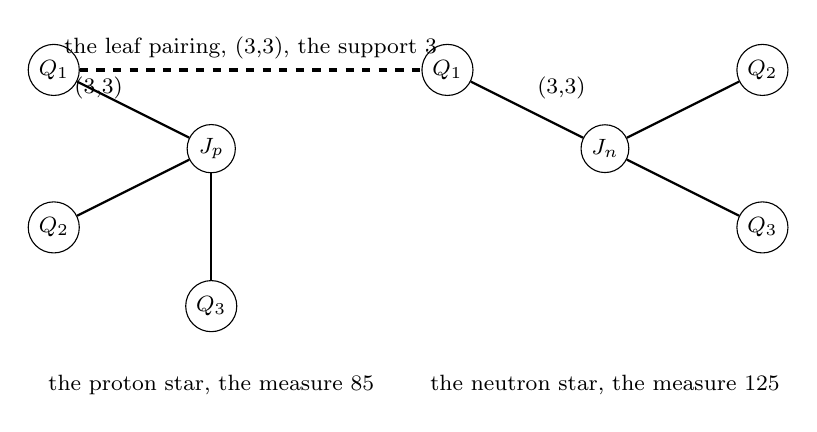
\begin{tikzpicture}[every node/.style={font=\footnotesize}]
\node[circle,draw,inner sep=2pt] (Jp) at (0,0) {$J_p$};
\node[circle,draw,inner sep=2pt] (p1) at (-2,1) {$Q_1$};
\node[circle,draw,inner sep=2pt] (p2) at (-2,-1) {$Q_2$};
\node[circle,draw,inner sep=2pt] (p3) at (0,-2) {$Q_3$};
\node[circle,draw,inner sep=2pt] (Jn) at (5,0) {$J_n$};
\node[circle,draw,inner sep=2pt] (n1) at (3,1) {$Q_1$};
\node[circle,draw,inner sep=2pt] (n2) at (7,1) {$Q_2$};
\node[circle,draw,inner sep=2pt] (n3) at (7,-1) {$Q_3$};
\draw[thick] (Jp) -- node[above left] {(3,3)} (p1); \draw[thick] (Jp) -- (p2); \draw[thick] (Jp) -- (p3);
\draw[thick] (Jn) -- node[above right] {(3,3)} (n1); \draw[thick] (Jn) -- (n2); \draw[thick] (Jn) -- (n3);
\draw[very thick,dashed] (p1) -- node[above] {the leaf pairing, (3,3), the support 3} (n1);
\node at (0,-3) {the proton star, the measure 85}; \node at (5,-3) {the neutron star, the measure 125};
\end{tikzpicture}
\caption{The deuteron as the two-star web. The proton star with its center $J_p$ of dimension three and three leaves, two of them pairable, and the neutron star with one pairable leaf, joined at the leaf pairing on the support three (the port face, the register $81$). The docks and arms of the stars are not drawn.}
\end{figure}
\section{The deuteron read at the shared typing}\label{mod:IX-6-D539124-w-kshd}
The deuteron is the one bound state of a proton and a neutron, a shallow bound state whose binding energy is small against the nucleon mass and whose wave function is dominated by the spin-triplet channel with a small tensor admixture; its properties follow from the nucleon-nucleon potential, in modern treatments the potential of a chiral effective theory \cite{Bethe1935,Weinberg1991}. Binding as the pairing records is introduced at section~\ref{mod:IX-6-binding-as-the-pairing-records-the-deuteron-and-the-alpha} and the body-alone office rule at section~\ref{mod:VIII-2-body-alone-office-rule}.
Under the shared passage typing of the measuring-path result at every link beyond the entry, with the geodesic through the pairing to the hub of the located arm, the records of the arm alone and the far-end count, the measuring read at the joined deuteron reads the proton first power plus two records at the leaf out-leg of the arm hub: the count 2873 equals the composed target of the established values, the first power as the segment sum, 319 multiplied by 9 plus 2, equals the product-plus-two spelling, and the office at that read is the pair part 8254129 plus the closure 6137 over 116640000 plus 1 over 48600 root 2.
The arm is exactly one uncapped link of two records passed by the read, and the office follows at the copied body-alone computations. But the first clause of the read, the typing of the links, is fixed by no established result: the typing of the arm is named rather than discharged at the premise census, the geodesic and the tie are named beside, and the count alone is discharged; so the read at the shared typing is an output of the established results at its count, its first power and its office and not at its typing clause, the parting between two cap results at the typing of the leaf links standing.
The result is an open result: the additive two of the neutron is an output of the one rule at the typing the measuring-path result lays at the leaf links and not at the typing the cap census lays, the first clause open and named; no comparison with observation enters its grade.
What stays open is the typing clause; the neutron closure at its own typing awaits its place in the compendium, and the alpha at this chapter stands at its own sections.
\par\medskip\noindent{\itshape Binding read, the next chapter lays out the nuclear rows.}\label{narr:close:9-6}\par
\section{The nuclear rows at the joined seeded web}\label{mod:IX-7-nuclear-rows-at-the-joined-seeded-web}
\chdesig{12-7}{9-7}{IX-7-nuclear-rows-at-the-joined-seeded-web}{IX-7-nuclear-rows-at-the-joined-seeded-web}
\label{narr:open:9-7}Open result~216.1 reads the nuclear rows at the joined seeded web as an open result, resting on the moves, the saturation and the binding chapter.
\begin{chwall}[The nuclear rows at the joined seeded web]\label{box:IX-7-nuclear-rows-at-the-joined-seeded-web:1}
The proton sink of the bound-respecting seed joined with the neutron twin at the dock pairing of the many-body readout, at the admission reading on the up docks alone, saturates under the pairing move at the second wave to one sink of the neutral kind at two open docks, whose binding entry at the two (2,2) pairing links reads its records at the first-power and Born-face entries by the derived genre cells. Face A, the made kind and the binding entry one object across the joined seeded web and the deuteron precedent, is unmet. Of nine compared fields the two entry words alone agree. Face B is met, and the parting is named with both objects. The first field, the pairing genre, reads (2,2) at the dock pairing of the seeded sinks against (3,3) at the leaf pairing of the deuteron, the records 57 against 412, the one-exchange 30 against 200, the two-exchange 3 against 28, the made kind neutral against beyond-two and the link register 16 against 81, so the question stays open.
\end{chwall}
\chstanding{open result}
\chdeps{Definitions 1.1 to 1.6, Open results 214.1 to 214.6, Open results 241.1 and 241.2, Theorems 241.3 and 241.4 and Open results 241.5 to 241.7 and Open results 245.1 and 245.2, Theorem 245.3, Open results 245.4 to 245.8 and Theorem 245.9}{no theorem beyond it at this release}
The joined seeded web is admitted at the dock pairing, saturated under the pairing move at the second wave to one sink, its binding entry printed as the pairing records at the established genre cells and compared with the deuteron precedent at nine fields, parting at the first. The results it rests on, the proton-web seeds, the bound-respecting seed, the many-body readout, the pairing move within a web and the direct two-exchange sum at the deuteron, are read as they stand. The register count is re-met at a second computation at all but eighteen of the webs of the closure, where the integers of that computation overflow while those of the first do not, a reading disclosed with the result, the deciding letter equal at both computations. What stands open is the parting itself, the nucleus results of the compendium standing at the open questions of the previous chapter.
\begin{chbridge}
In the standard account a nucleus is a bound state of protons and neutrons held by the residual strong force, its binding read at the semi-empirical mass formula and its structure at the shell model with the magic numbers of closed shells \cite{BetheBacher1936,Mayer1949}. The correspondence is by name.
\end{chbridge}
\begin{chproof}[exhaustive census]
\textit{The premises.} The axiom and the six definitions of Section~\ref{mod:FRAMEWORK}, definitions. The moves of Section~\ref{mod:I-4-moves-in-one-table}, definitions. The seeds, the waves and the sinks of Section~\ref{mod:I-5-saturation-in-one-figure-seeds-waves-termination-sinks}, a theorem. The binding as the pairing records of Section~\ref{mod:IX-6-binding-as-the-pairing-records-the-deuteron-and-the-alpha}, an open result. The proton-web seeds, the bound-respecting seed, the many-body readout and the pairing move within a web, open results read as they stand. The chain from the axiom to this result is six chapters deep.

\textit{The census.} The set counted is the joined webs reached from the two seeded sinks apart under the pairing move at the dock pairing, generated wave by wave to the stop condition (a sink where no pairing move extends the web). The two seeded sinks are the proton sink of the bound-respecting seed (eight sites, nine links, the measure $81$, three open docks) and the neutron twin (twelve sites, fourteen links, the measure $121$, the arm turned down as the library spells the down web). At the admission reading on the up docks alone, nine unlike dock pairs of which six are admitted, the saturation reaches three webs over the waves $0{:}1$, $1{:}1$, $2{:}1$ and stops at one sink at the second wave, with twenty sites, twenty-five links, the measure $210$, the dressing $12$, the genre census $(2,2){:}3$, $(2,3){:}6$, $(2,4){:}3$, $(3,3){:}6$, $(3,4){:}7$, its made kind neutral at two open docks. The property tested at the sink is its binding entry at the two (2,2) pairing links by the derived genre cells. The entry carries the records $57$ per link, the one-exchange $30$, the two-exchange $3$, the records the pairing adds $114$, the order-one count
\begin{equation}
60\cdot(2\cdot 5250-60)=626\,400
\end{equation}
entering at the first-power entry (the one-exchange total $5250$ of the joined sink against $5190$ of the two sinks apart), and the order-two count $6$ entering at the Born-face entry. Against the deuteron entry, the leaf pairing at the genre (3,3) with the records $412$, the one-exchange $200$, the two-exchange $28$, the order-one count $200\cdot(2\cdot 5162-200)=2\,024\,800$ and the order-two count $28$, the nine compared fields agree at 2 of 9, the two entry words, and part first at the pairing genre. The first parting element is that field, (2,2) against (3,3). Beside, at the admission reading on any dock the saturation reaches six webs and a sink of the dark kind at the third wave, and the pair of two proton sinks four webs and a dark sink. Every joined web is a sink of the preceding census, and the register count is re-met at 101\,973 of 101\,973 webs of the site-bounded closure at the first computation. The smallest case is the one-pairing web, with the records $57$, the order-one count $311\,400$ and the order-two count $3$, checked by hand from the formula.

\textit{The check.} Joining at the hub legs instead moves the pairing genre, the records and the order-two count. Striking the saturation leaves the one-pairing web of the beyond-two kind in place of the neutral sink. Each alteration moves the cells it names. The result was reproduced by an independent route, two computations of different construction agreeing at the deciding letter and at every cell of the item, the second overflowing at eighteen webs of the closure far above the registers of this item.
\chcert{101973}
\end{chproof}
\par\medskip\noindent{\itshape The Part closes on the processes held as a table.}\label{narr:close:9-7}\par
